%%%%%%%%%%%%%%%%%%%%%%%%%%%%%%%%%%%%%%%%%%%%%%%%%%%%%%%%%%%
%\documentclass[xcolor=x11names,compress]{beamer}
\documentclass[xcolor=x11names,compress, aspectratio=169]{beamer}
%% General document
\usepackage{graphicx, subfig}
%% Beamer Layout
\useoutertheme[subsection=false,shadow]{miniframes}
\useinnertheme{default}
\usefonttheme{serif}
\usepackage{palatino}

%%%%%%% Mes Packages %%%%%%%%%%%%%%%%
%\usepackage[french]{babel}
\usepackage[T1]{fontenc}
\usepackage{color}
\usepackage{xcolor}
\usepackage{dsfont} % Pour indicatrice
\usepackage{url}
\usepackage{multirow}
\usepackage[normalem]{ulem}   % For strike out text

% Natbib for clean bibliography
\usepackage[comma,authoryear]{natbib}

%remove the icon
\setbeamertemplate{bibliography item}{}

%remove line breaks
\setbeamertemplate{bibliography entry title}{}
\setbeamertemplate{bibliography entry location}{}
\setbeamertemplate{bibliography entry note}{}

%% ------ MEs couleurs --------
\definecolor{vert}{rgb}{0.1,0.7,0.2}
\definecolor{brique}{rgb}{0.7,0.16,0.16}
\definecolor{gris}{rgb}{0.7, 0.75, 0.71}
\definecolor{twitterblue}{rgb}{0, 0.42, 0.58}
\definecolor{airforceblue}{rgb}{0.36, 0.54, 0.66}
\definecolor{siap}{RGB}{3,133, 200}


%%%%%%%%%%%%%%%%% BEAMER PACKAGE %%%%%%%

\setbeamercolor{itemize item}{fg=siap}
%\setbeamercolor{itemize subitem}{fg=blue}
%\setbeamercolor{itemize subsubitem}{fg=cyan}

\setbeamerfont{title like}{shape=\scshape}
\setbeamerfont{frametitle}{shape=\scshape}

\setbeamercolor*{lower separation line head}{bg=DeepSkyBlue4}
\setbeamercolor*{normal text}{fg=black,bg=white}
\setbeamercolor*{alerted text}{fg=siap}
\setbeamercolor*{example text}{fg=black}
\setbeamercolor*{structure}{fg=black}
\setbeamercolor*{palette tertiary}{fg=black,bg=black!10}
\setbeamercolor*{palette quaternary}{fg=black,bg=black!10}

% Set the header color to SIAP's color
\setbeamercolor*{frametitle}{fg=siap}

%remove navigation symbols
\setbeamertemplate{navigation symbols}{}

\renewcommand{\(}{\begin{columns}}
\renewcommand{\)}{\end{columns}}
\newcommand{\<}[1]{\begin{column}{#1}}
\renewcommand{\>}{\end{column}}

%% Add footer with logo
\setbeamertemplate{footline}{%
  \begin{beamercolorbox}[wd=\paperwidth,ht=2.5ex,dp=1.125ex,%
    leftskip=.3cm,rightskip=.3cm plus1fil]{author in head/foot}
    
\includegraphics[height=5ex]{SIAP_logo_Big.png}\hfill
    \insertshortauthor\hfill\insertshorttitle\hfill  \textcolor{siap}{\textit{\insertframenumber}}
  \end{beamercolorbox}%
}


% Path for the graphs
\graphicspath{
{Graphics/}
{c:/Chris/Visualisation/Presentations/Graphics/Logos}
{c:/Chris/Visualisation/Presentations/Graphics/}
{c:/Chris/Visualisation/Presentations/Graphics/Lies/}
{c:/Chris/Visualisation/Presentations/Graphics/Uncertainty/}
{c:/Gitmain/MLCourse/UNML/Module0/M0_files/figure-html/}
{c:/Chris/UN-ESCAP/MyCourses2022/MLOS2022/Slides/Graphics/}
{c:/Chris/UN-ESCAP/MyCourses2023/BigDataKostat/Slides/Graphics/}
{c:/Chris/Visualisation/Presentations/Graphics/SIAP/icons/}
{c:/Chris/UN-ESCAP/SIAP-E-learning/Resources/Pictos/}
{c:/Chris/UN-ESCAP/MyCourses/DataViz/R-Codes/M5-Maps_files/figure-latex/}
{c:/Chris/UN-ESCAP/MyCourses/DataViz/Graphics/}
{c:/Chris/UN-ESCAP/MyCourses/DataViz/Graphics/}
{c:/Chris/UN-ESCAP/MyCourses/DataViz/Graphics/FromPdf/}
{c:/Chris/UN-ESCAP/MyCourses/DataViz/R-Codes/JobSatisfaction_files/figure-latex/}
{c:/Chris/UN-ESCAP/MyCourses/DataViz/R-Codes/Unused_files/figure-latex/}
{c:/Chris/UN-ESCAP/MyCourses/DataViz/R-Codes/M2-DataInkRatioBoxplot_files/figure-latex/}
{c:/Chris/UN-ESCAP/MyCourses/DataViz/R-Codes/Unused_files/figure-latex/}
{c:/Chris/UN-ESCAP/MyCourses/DataViz/R-Codes/M4-VisualizingManyDimensions_files/figure-latex/}
{c:/Chris/UN-ESCAP/MyCourses2023/AdvancedDataVisualization/Slides/Graphics/}
 }

\title{\textcolor{siap}{Big Data and Data Science for Gender Statistics in Asia and the Pacific\\ \vspace{0.5cm} }}

\subtitle{\textcolor{brique}{\Large{Data Visualization for Gender Statistic }}}
\author{Christophe Bontemps}
\institute{ 
\includegraphics[height=10ex]{SIAP_logo_Big.png}}
\date{}


\begin{document}

% Slide 1: Title Slide
\begin{frame}
    \titlepage
\end{frame}


%%%%%%  Path for the graphs
%\graphicspath{
%{Graphics/}
%{../../../../Visualisation/Presentations/Graphics/}
%{../../Visualisation/Presentations/Graphics/}
%{c:/Gitmain/MLCourse/UNML/Module0/M0_files/figure-html/}
%{c:/Chris/UN-ESCAP/MyCourses2022/MLOS2022/Slides/Graphics/}
%{c:/Chris/UN-ESCAP/SIAP-E-learning/Resources/Pictos/}
%%%%%
%{../Graphics/}
%{../../../../Visualisation/Presentations/Graphics/}
%{../../../../Visualisation/Presentations/Graphics/Lies/}
%{../../../../Visualisation/Presentations/Graphics/SIAP/}
%{c:/Chris/UN-ESCAP/MyCourses/DataViz/Graphics/}
%{c:/Chris/UN-ESCAP/MyCourses/DataViz/Graphics/FromPdf/}
%{c:/Chris/UN-ESCAP/MyCourses/DataViz/R-Codes/JobSatisfaction_files/figure-latex/}
%{c:/Chris/UN-ESCAP/MyCourses/DataViz/R-Codes/Unused_files/figure-latex/}
%{c:/Chris/UN-ESCAP/MyCourses/DataViz/R-Codes/M2-DataInkRatioBoxplot_files/figure-latex/}
%{c:/Chris/UN-ESCAP/MyCourses/DataViz/R-Codes/Unused_files/figure-latex/}
%{c:/Chris/UN-ESCAP/MyCourses/DataViz/R-Codes/M4-VisualizingManyDimensions_files/figure-latex/}
%{c:/Chris/UN-ESCAP/MyCourses2023/BigDataKostat/Slides/Graphics/}
% }


%%%%%% DTV Intro %%%%

\begin{frame} % Cover slide
\frametitle{\textcolor{brique}{[-Foreword-]}}
\begin{center}

\huge{\textcolor{siap}{What is Data Visualisation about?}}
\end{center}
\end{frame}


\begin{frame} % Cover slide
\frametitle{\textcolor{brique}{[-Foreword-]}: What's Data Visualisation?}
\begin{center}
What do you see?\\

  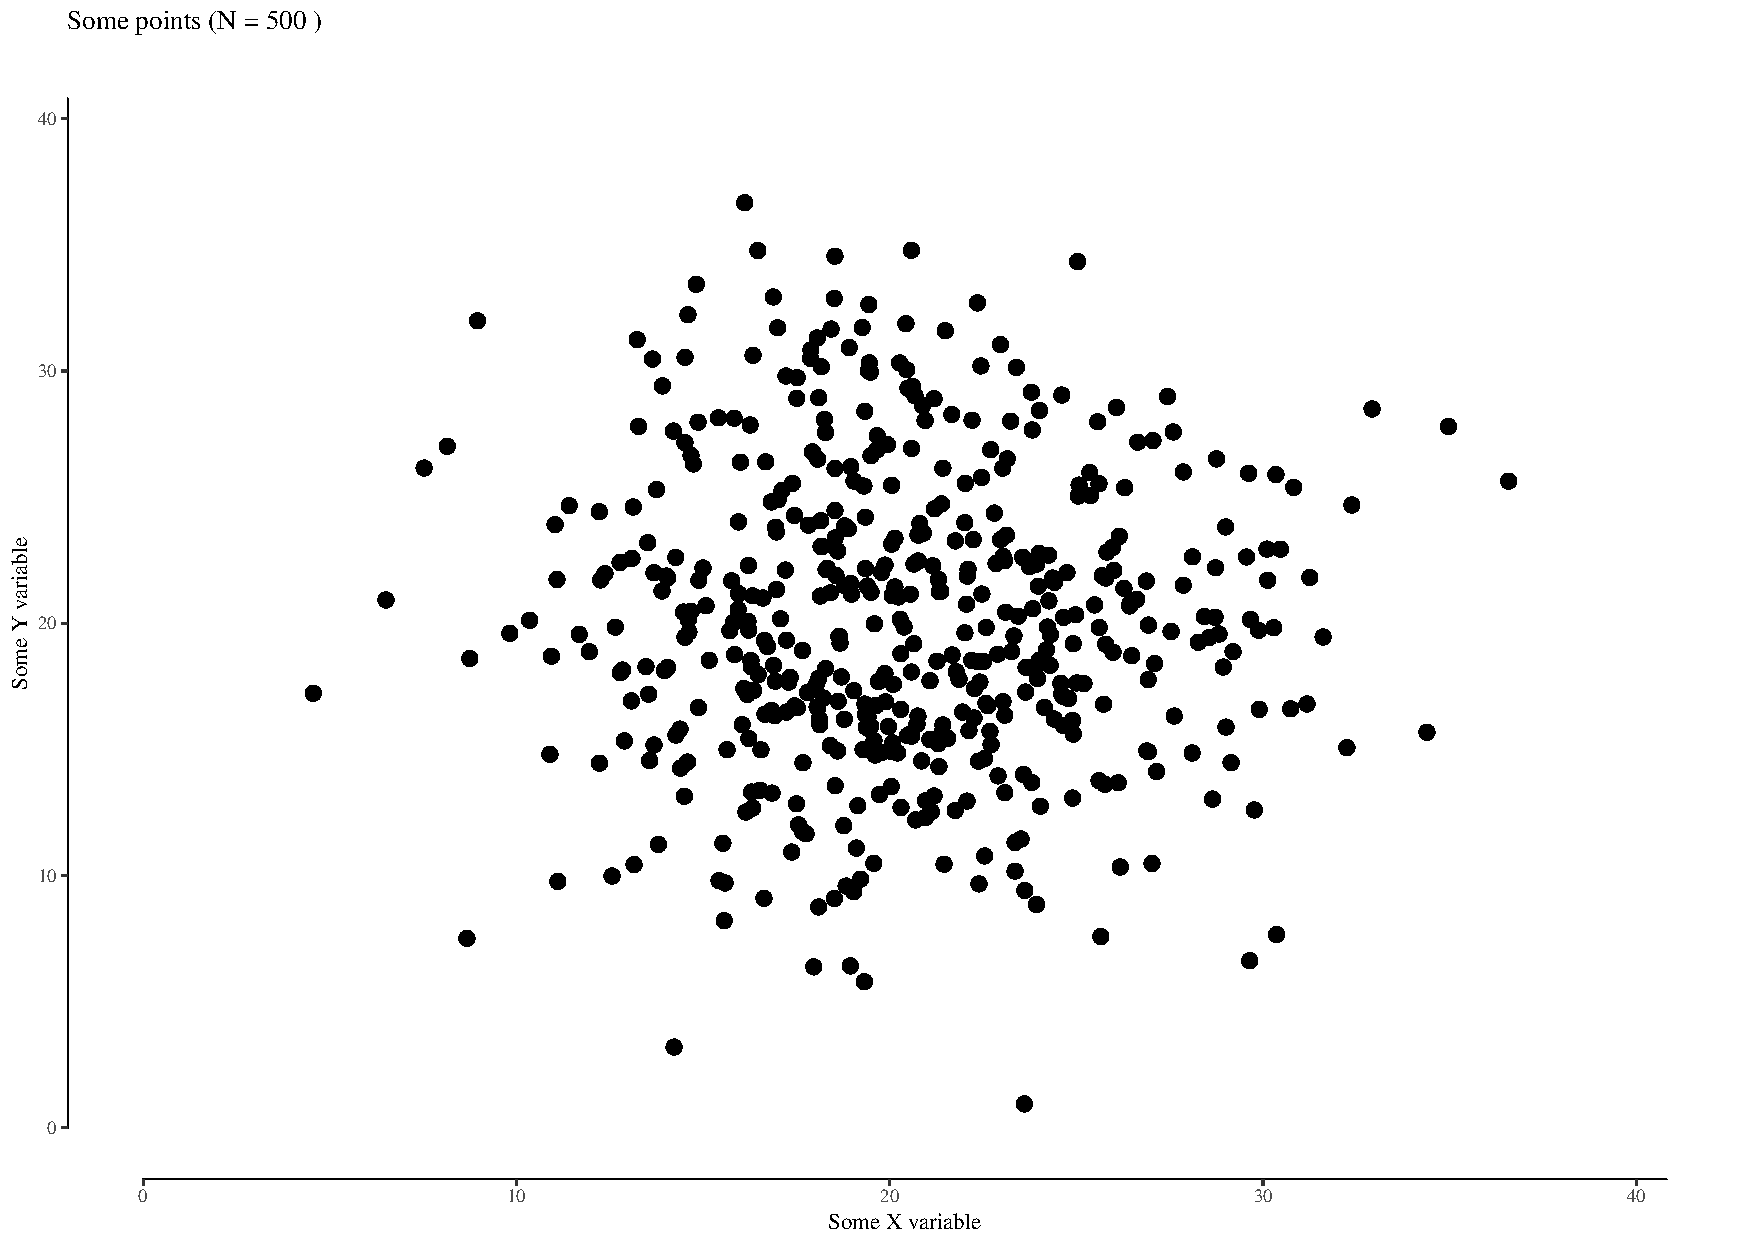
\includegraphics[width = 0.6\textwidth]{RandomPoints.pdf}
\end{center}
\end{frame}


\begin{frame} % Cover slide
\frametitle{\textcolor{brique}{[ - What Is Data Visualisation? - ]}}
 \begin{center}
 And here, what do you see?\\
  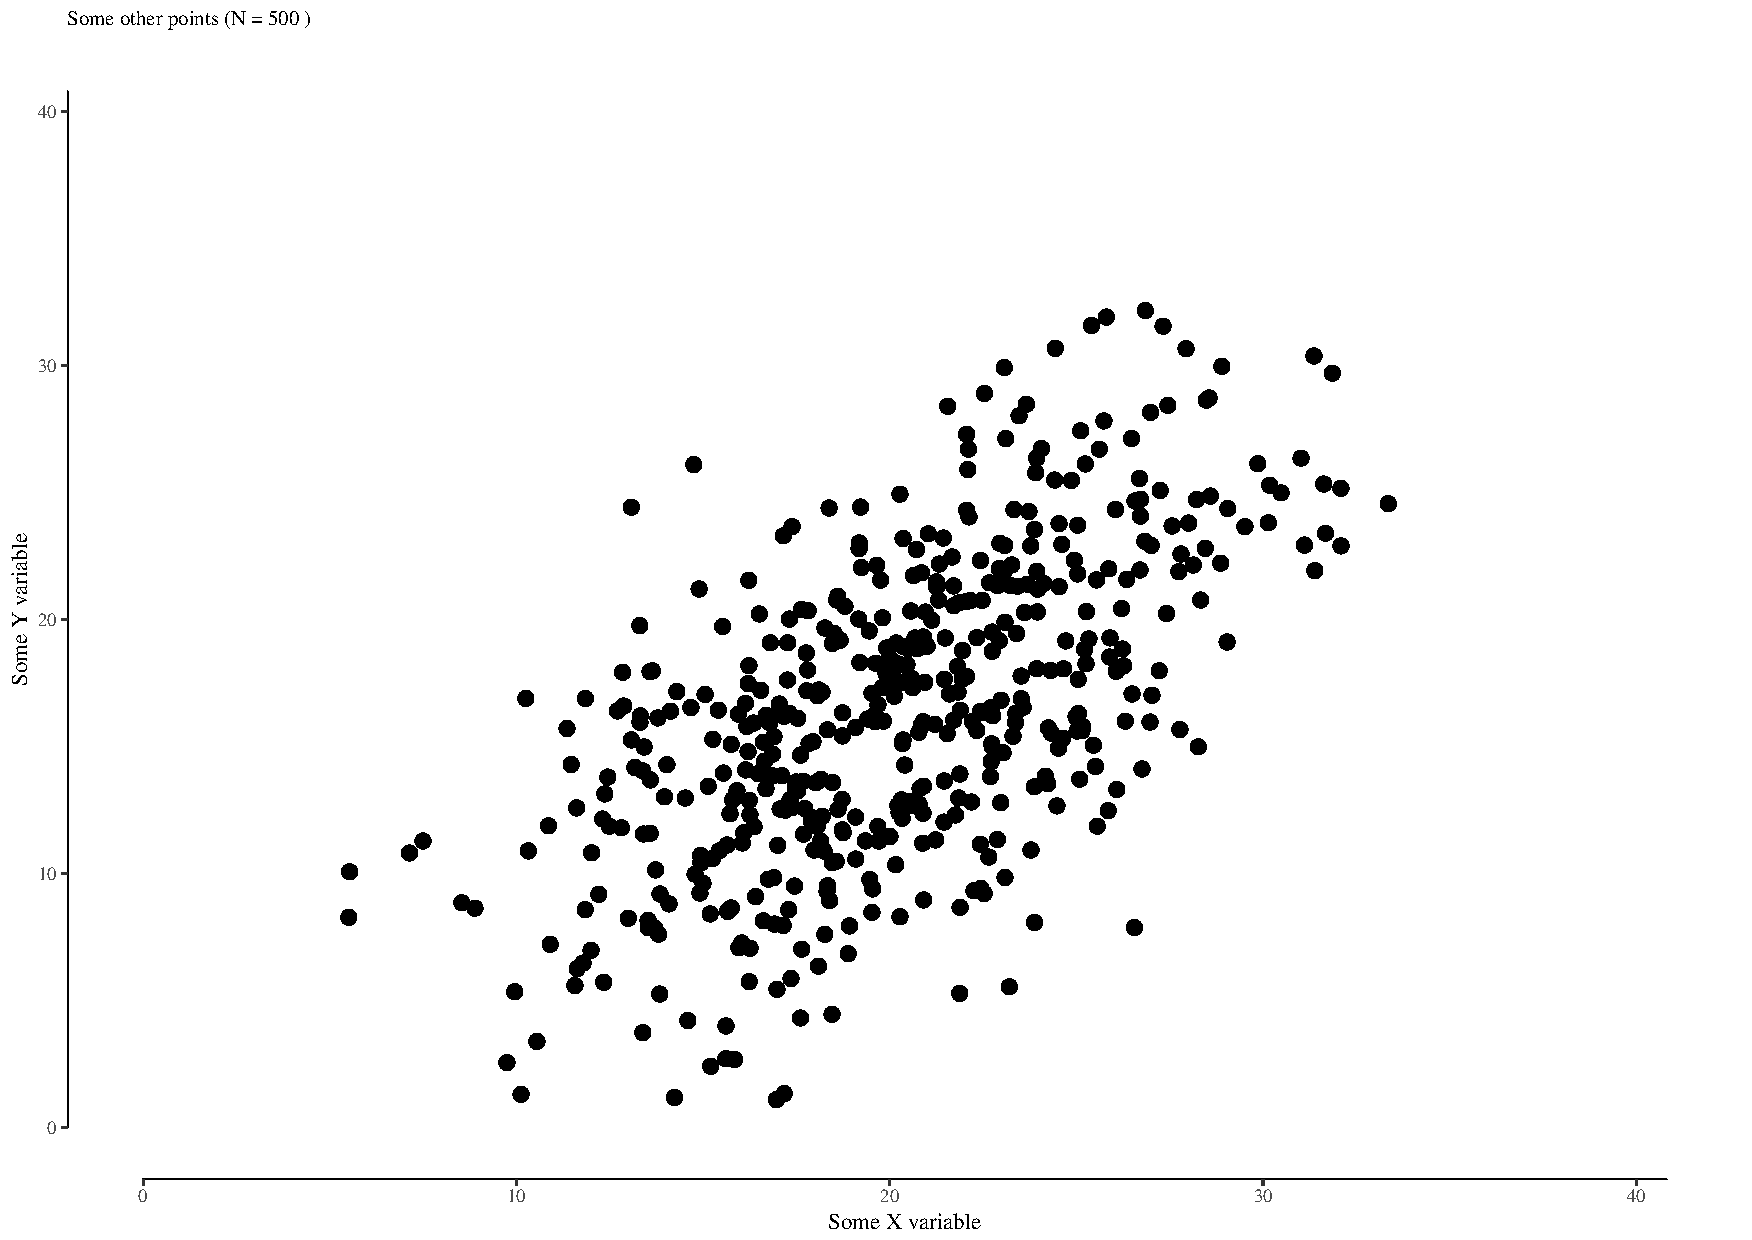
\includegraphics[width = 0.6\textwidth]{LinearPoints1.pdf}
\end{center}
\end{frame}

\begin{frame} % Cover slide
\frametitle{``Data visualisation'' as a statistical test }
 \begin{itemize}
  \item<+->[] 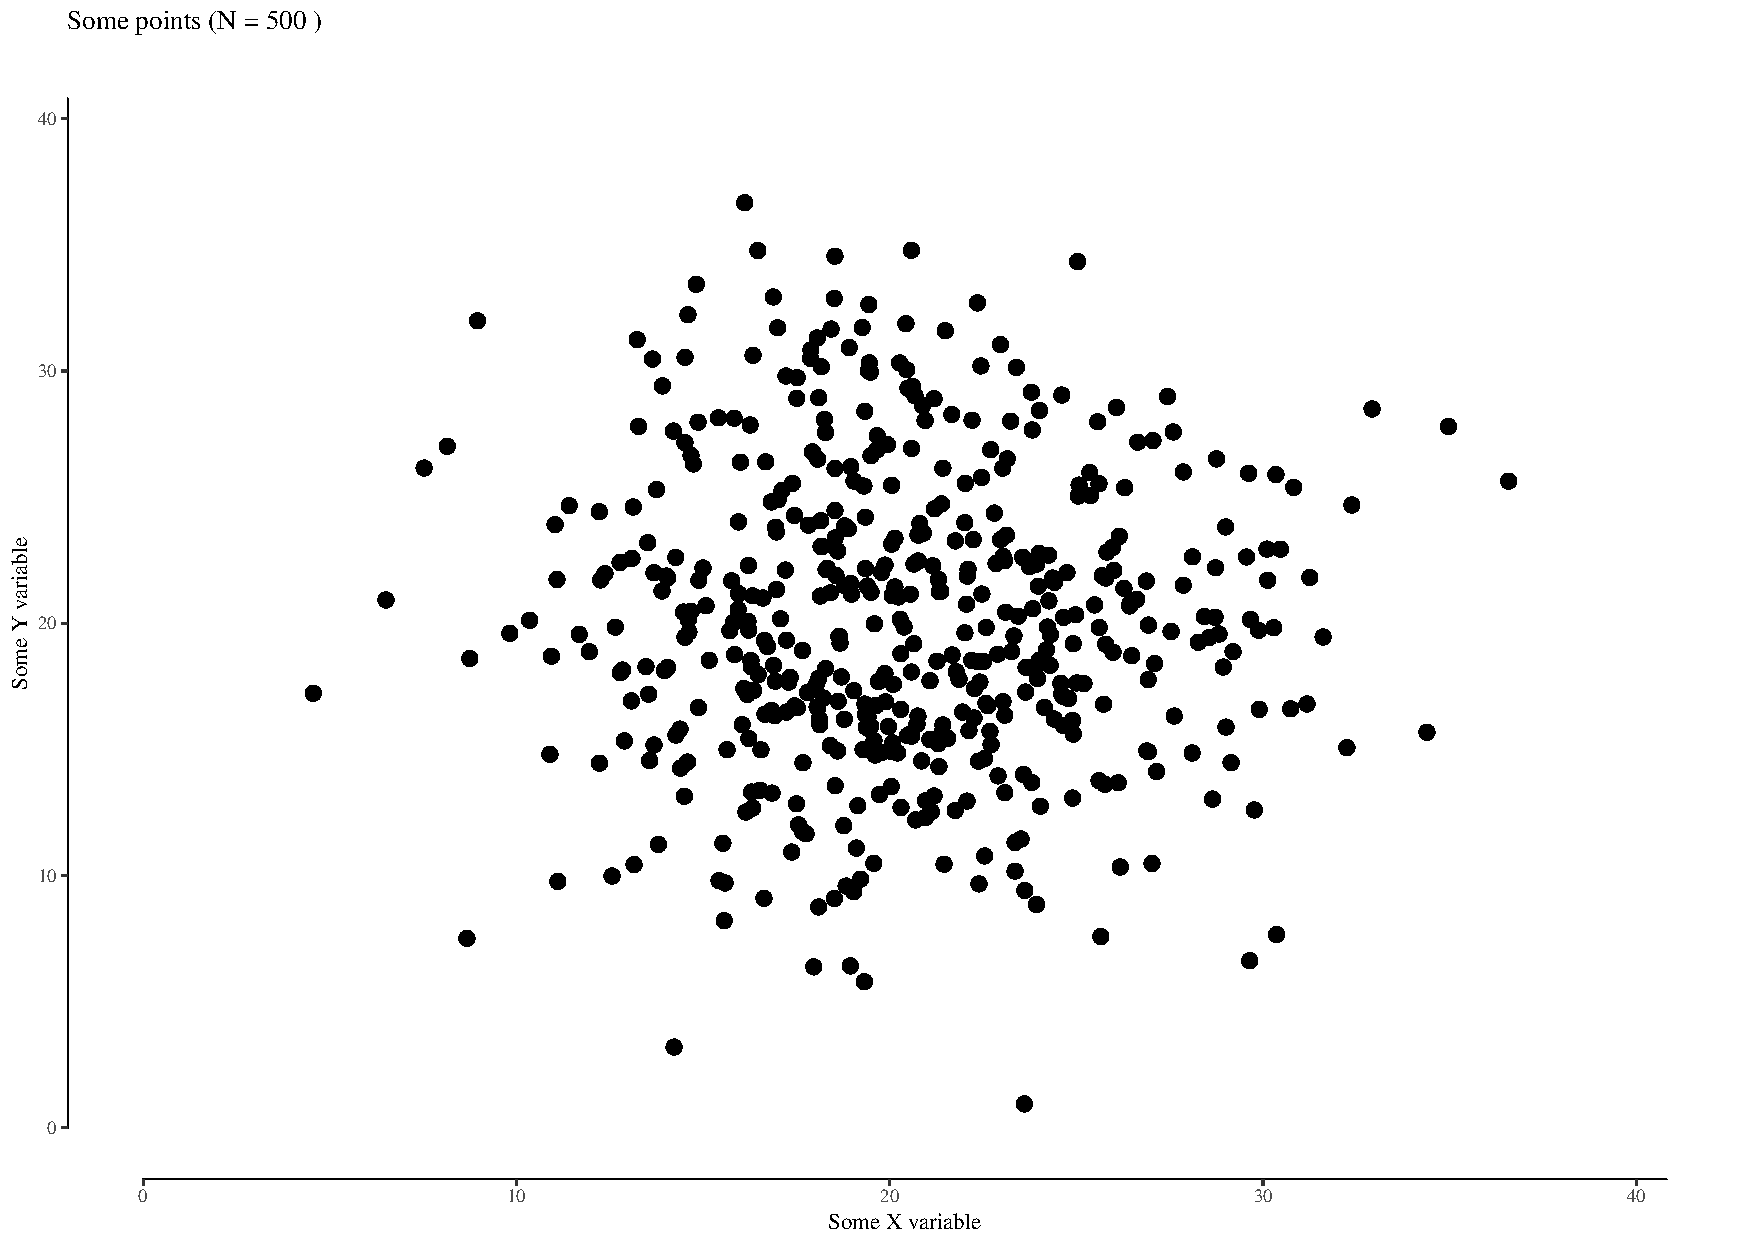
\includegraphics[width = 0.2\textwidth]{RandomPoints.pdf}
            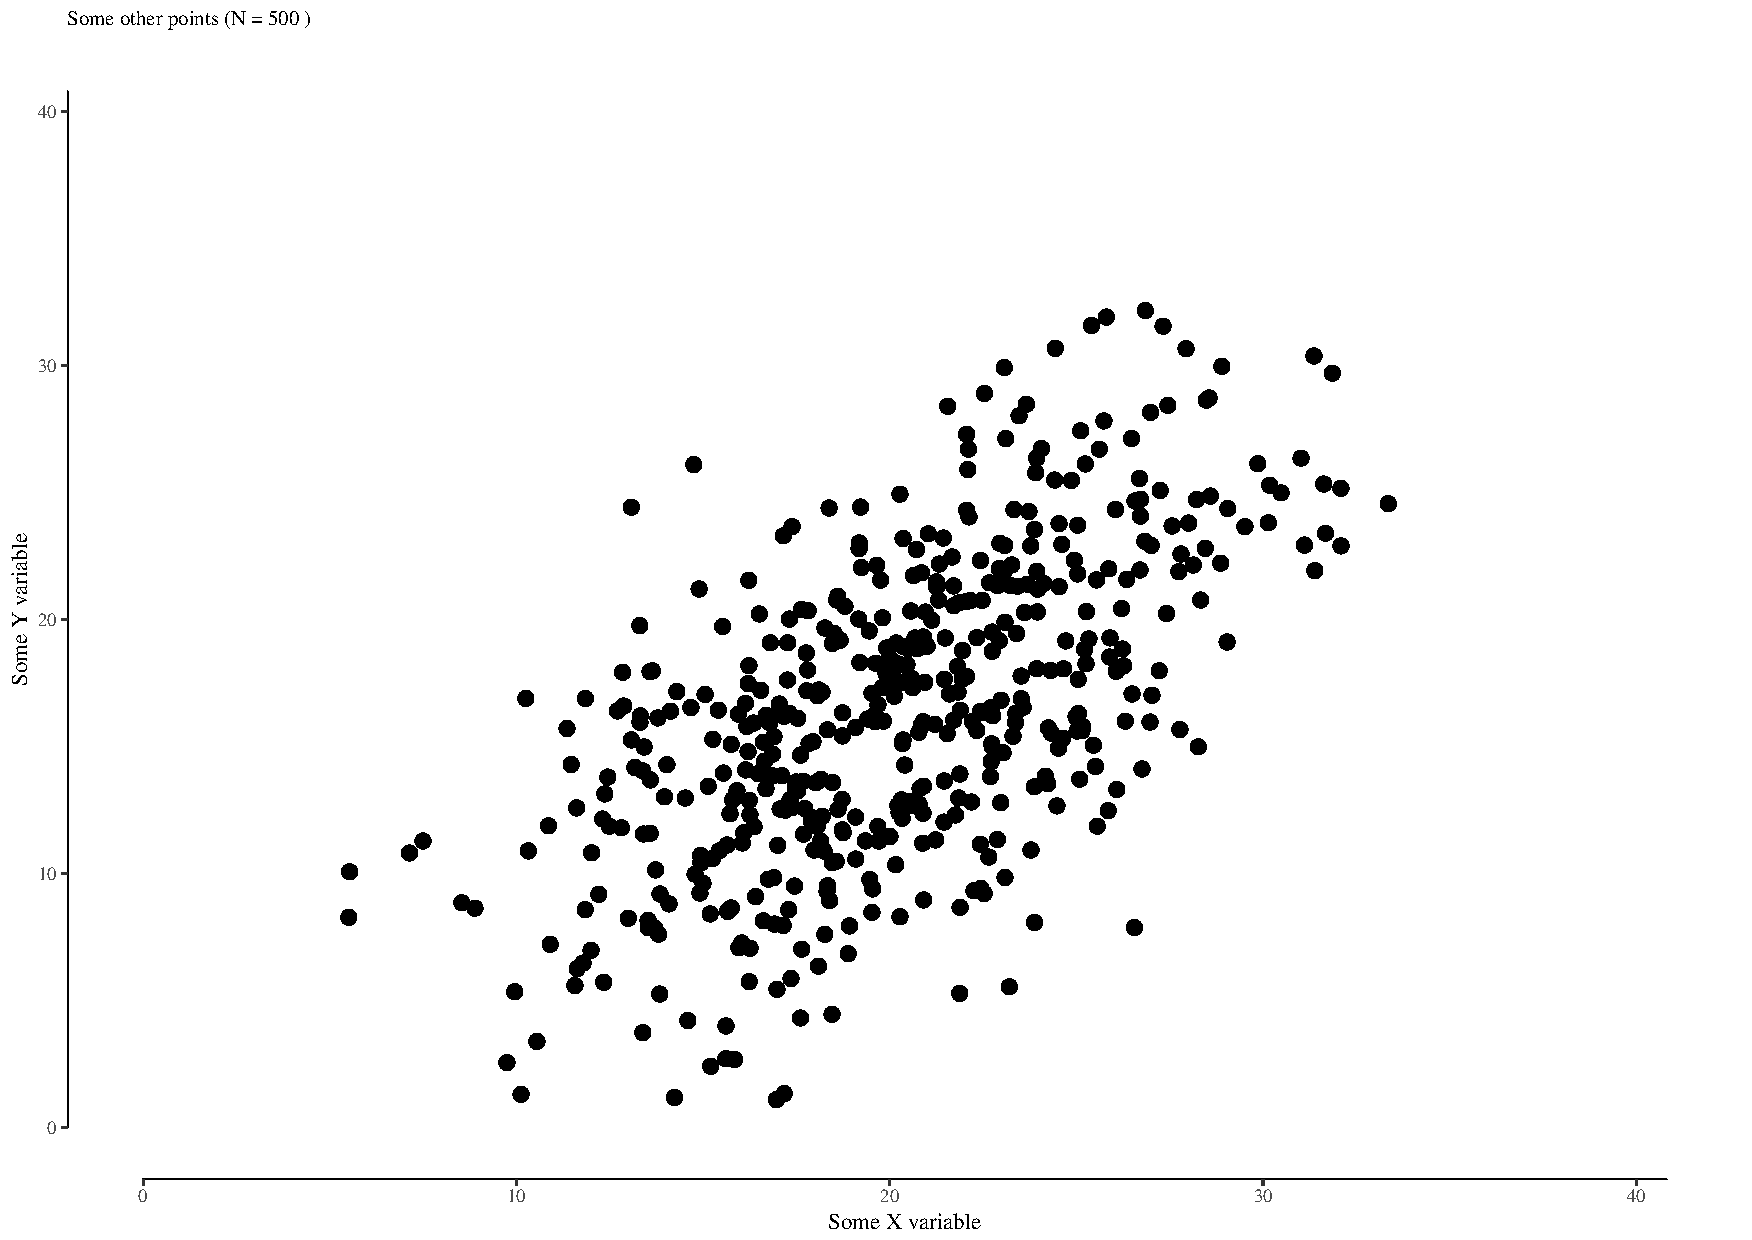
\includegraphics[width = 0.2\textwidth]{LinearPoints1.pdf}
            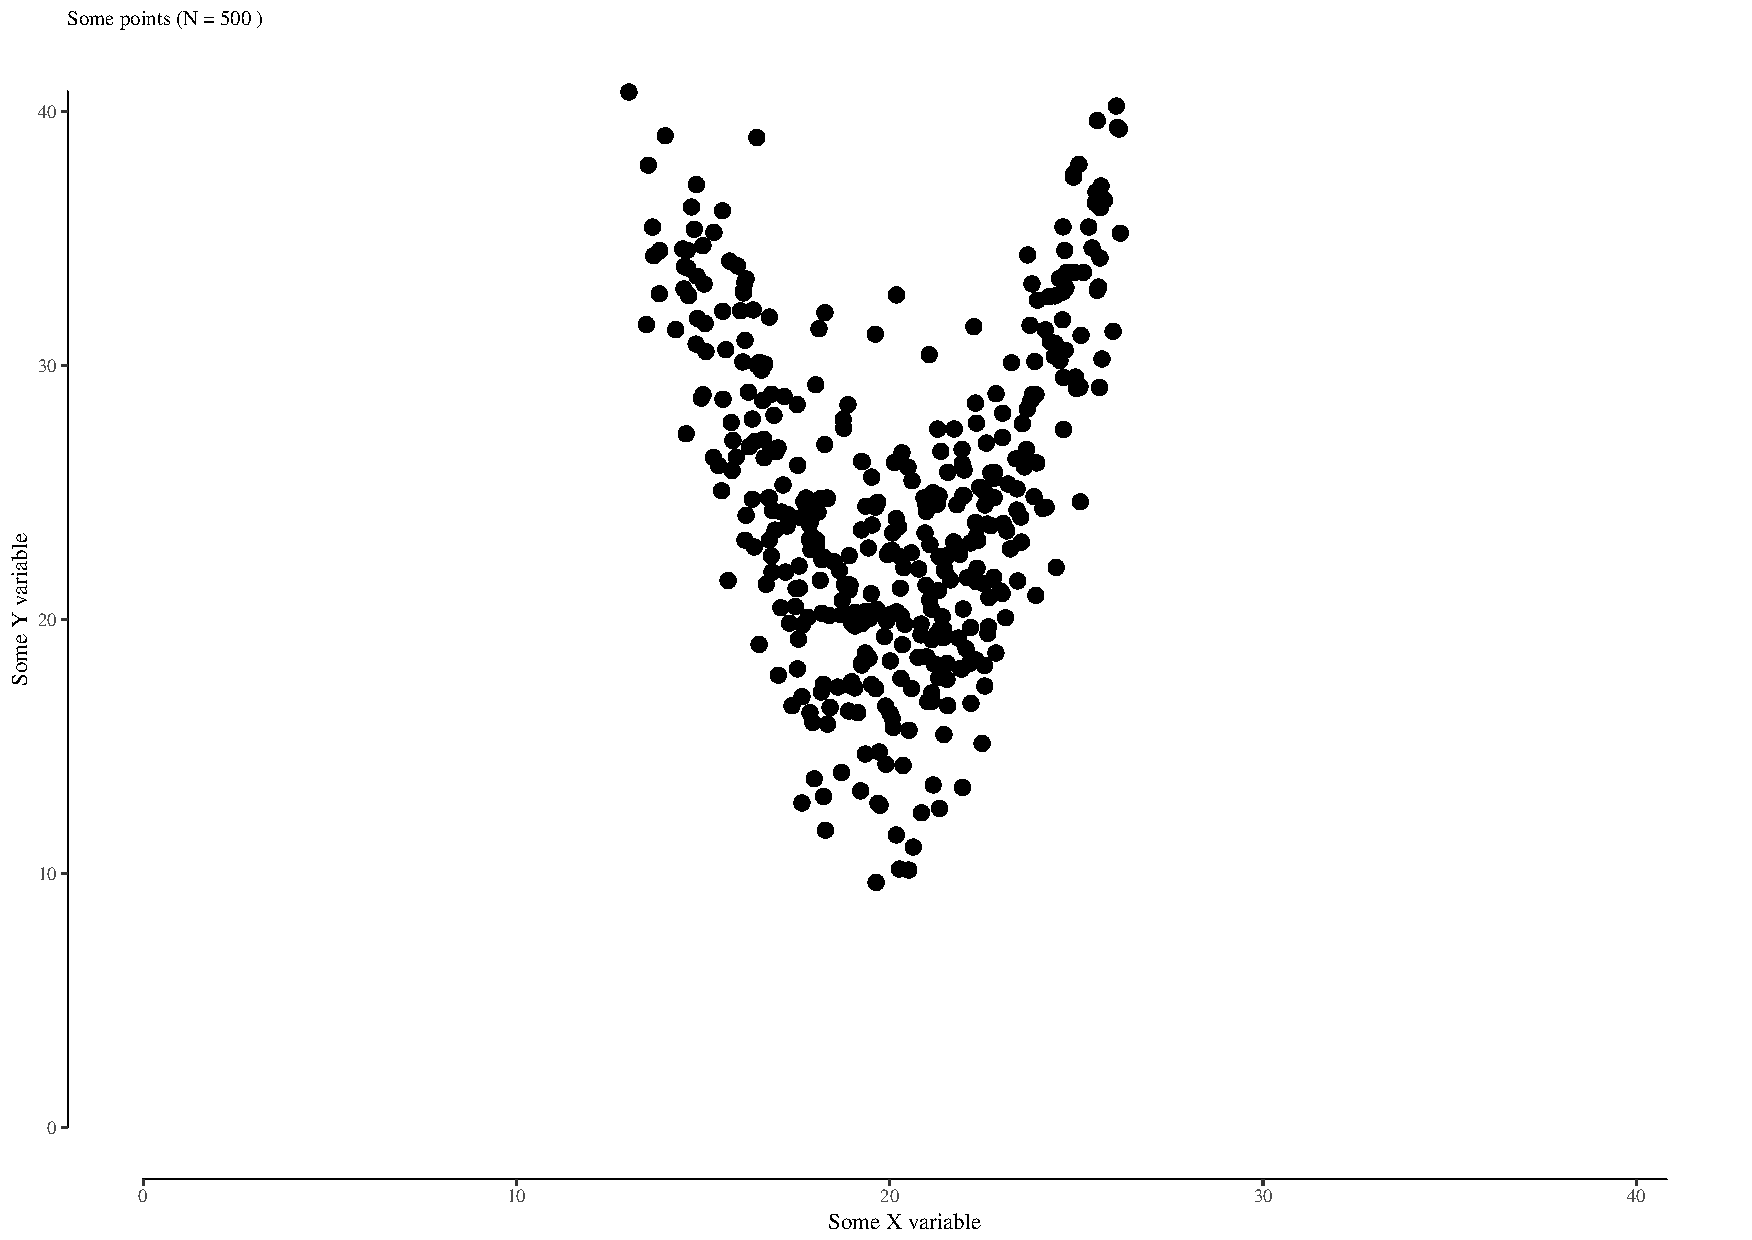
\includegraphics[width = 0.2\textwidth]{UshapedPoints.pdf}
            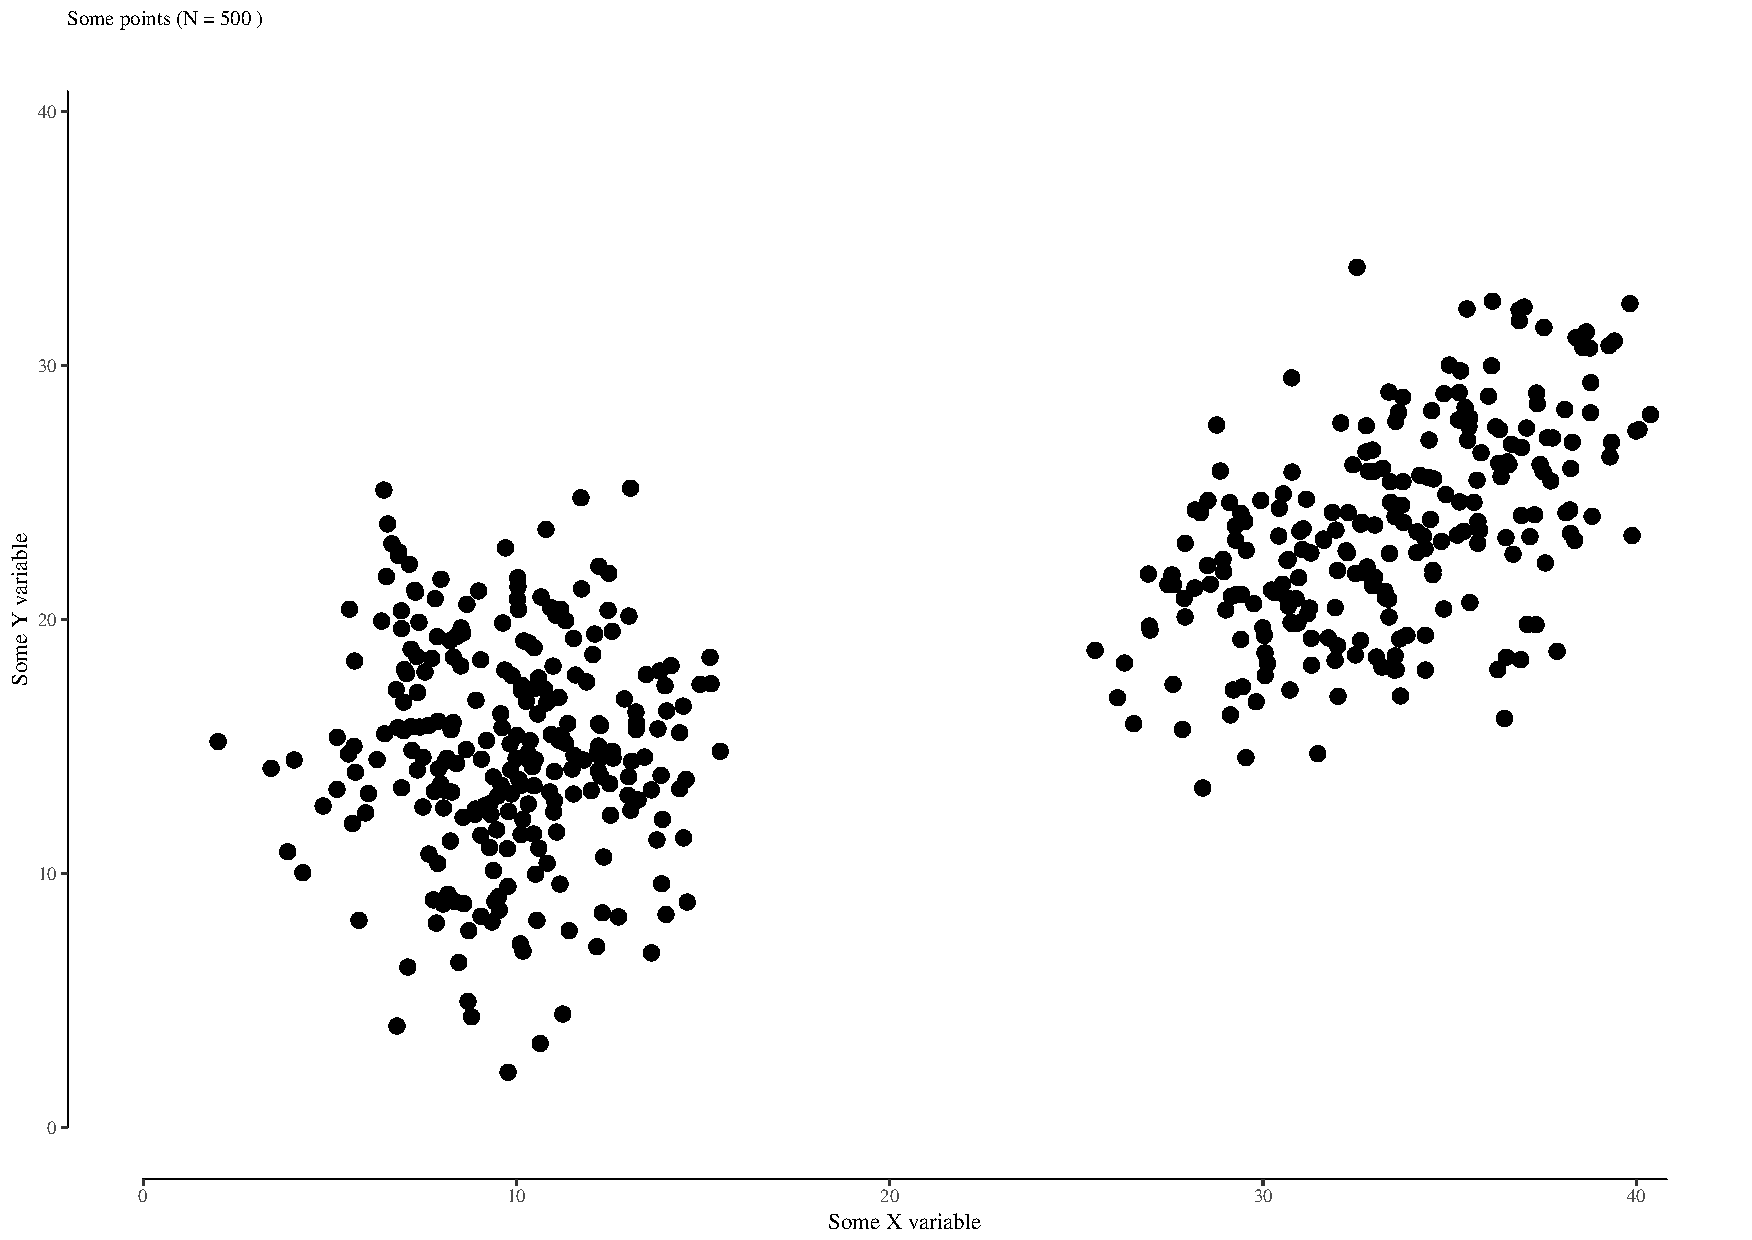
\includegraphics[width = 0.2\textwidth]{GroupsPoints.pdf}
  \item<+->[] {\centering \textit{`` The human eye acts is a broad feature detector and general statistical test''. \cite{Buja2009}}}
  \item<+->[\textbf{Test:}] $H_0$ : \{There is "nothing"  \} = \{\textbf{No} relation\}
  \item<+->[] $H_1$ : \{ There is "something" \} = \{There is \textbf{some} relation (Correlation, linearity, heterogeneity, groups..) \}
 \end{itemize}
\end{frame}

\begin{frame} % Cover slide
\frametitle{\textcolor{brique}{[-Foreword-]}: What's Data Visualisation?}
\begin{center}

\huge{\textcolor{siap}{Data Visualization is about\\   (fair!)} \textcolor{brique}{comparisons}}
\end{center}
\end{frame}

\begin{frame} % Cover slide
\frametitle{\textcolor{brique}{[- What we do: -]}: \textbf{Implicit} comparisons}
\begin{center}
\begin{itemize}
  \only<1>{What does this curves tells you ? }
  \only<1>{ 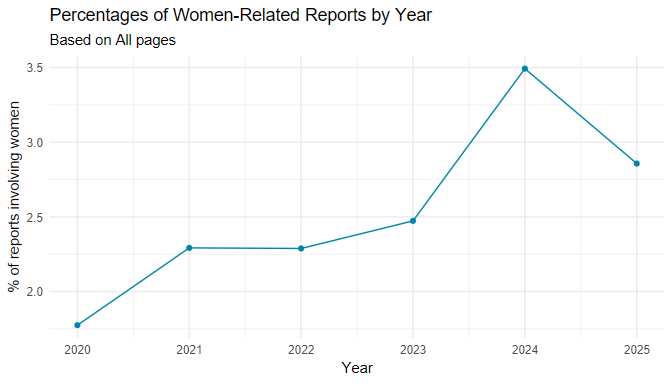
\includegraphics[width = 0.7\textwidth]{CurveUp.png}}
\end{itemize}
\end{center}
\end{frame}

\begin{frame} % Cover slide
\frametitle{\textcolor{brique}{[- What we do: -]}:  \textbf{Explicit} comparisons }

\begin{center}
\begin{itemize}
  \only<1>{We compare: \textcolor{brique}{\textbf{surfaces}... }}
  \only<1>{ 
\includegraphics[width = 0.7\textwidth]{DesignNumbers-18.png}}
  \only<2>{ \textcolor{brique}{\textbf{lines}... } \\ \vspace{0.5cm} }
  \only<2>{}
  \only<2>{ 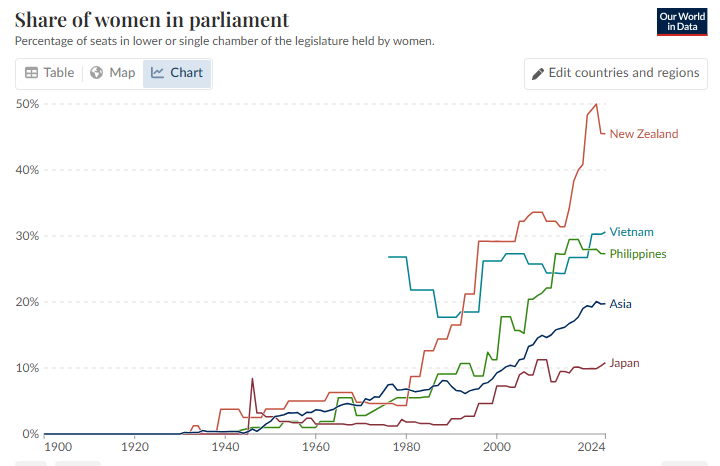
\includegraphics[width = 0.55\textwidth]{ShareWomenParliament-line.png}}
  \only<3>{\textcolor{brique}{\textbf{Bar lengths}...} \\ }
  \only<3>{ 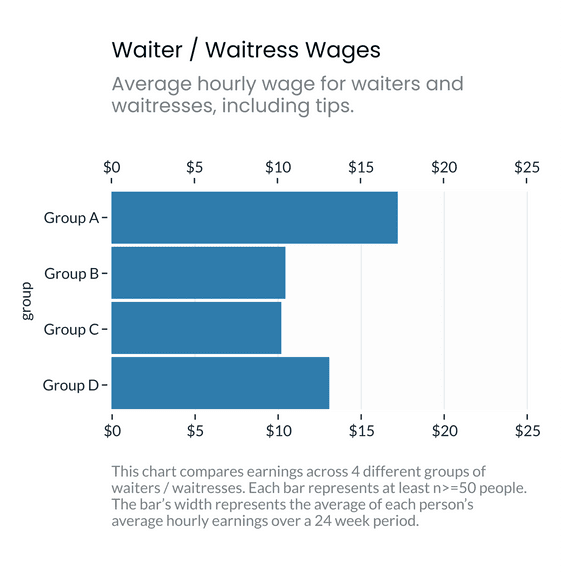
\includegraphics[width = 0.45\textwidth]{WaiterBar.png}}
  \only<4>{\textcolor{brique}{\textbf{colors}...}  \\ }
  \only<4>{ 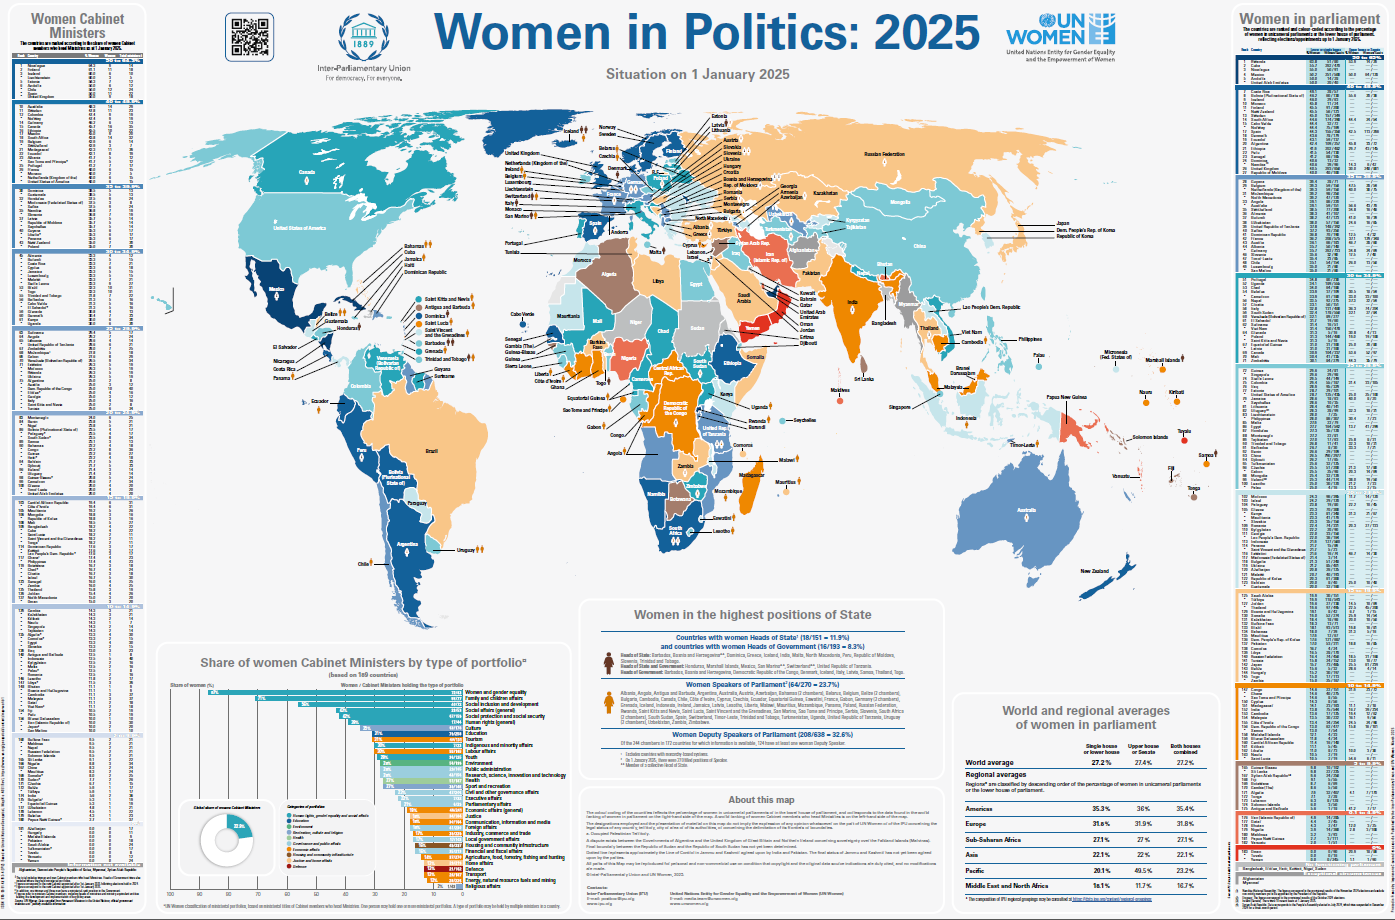
\includegraphics[width = 0.7\textwidth]{UNWomen-WomenPolitics2025.png}}
\end{itemize}
\end{center}
\end{frame}

%%%%% DTV-M4 Complexity    %%%%%%

\begin{frame}
\frametitle{\textcolor{brique}{[- \textbf{Visualizing in many dimensions} -]}}
\begin{center}
\begin{itemize}
   \item<+-> Real data are complex and in multiple dimensions
   \item<+-> Visualizing for data exploration is important % exploration vs presentation
   \item<+-> Analysing data one after another is not providing a good overview
   \item<+-> Visualizing multiple relationships is mandatory
   \item<+->  Difficult to compare many dimensions
\end{itemize}
\end{center}
\end{frame}

\begin{frame}
\frametitle{\textcolor{brique}{[- \textbf{Visualizing in many dimensions} -]}}
\begin{center}
\begin{itemize}
   \item<+->[]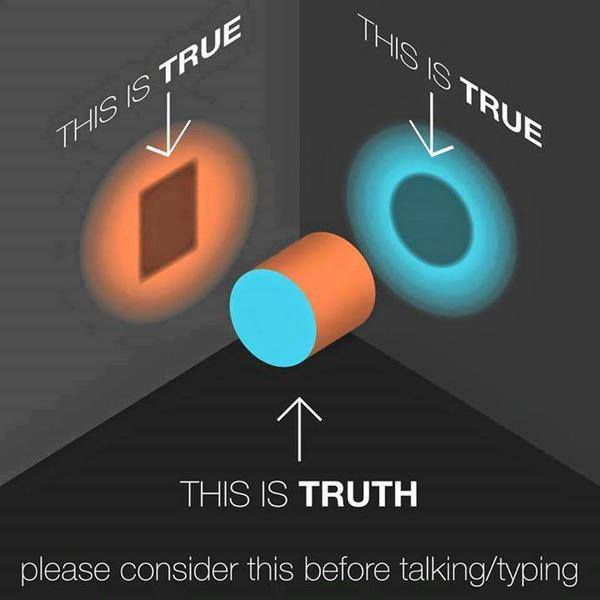
\includegraphics[width=0.4\textwidth]{TrueAndTrue.jpg}
\end{itemize}
\end{center}
\end{frame}


\section{Goals}

% the \setbeamercolor and the frame to limit the scope
{\setbeamercolor{background canvas}{bg=siap}
 \setbeamercolor{item}{fg=white}
    \setbeamercolor{normal text}{fg=white}
    \usebeamercolor[fg]{normal text}

\begin{frame}
\hspace{4cm}
\begin{center}
\Huge{Goals of Data Visualisation}
\end{center}
\end{frame}

} %end blue Background


%%%  ----------- Dataviz  Goals  -----------%%%

\begin{frame}
\frametitle{Goals of Data Visualisation}

\begin{itemize}
    \item<+->[]  Data visualisation serves \textit{at least} two main purposes:
    \item<+-> \textcolor{siap}{\textbf{Data exploration}} \\
    \item<+->[] Graphics as visual tests, \textcolor{brique}{comparisons}
   \item<+->[] $\rightarrow$ \textbf{short} time to built and to read
    \item<+-> \textcolor{siap}{\textbf{Data representation}}\\
    \item<+->[] Summaries, \textcolor{brique}{comparisons}, storytelling
     \item<+->[] $\rightarrow$ \textbf{long} time to build, short time to read
     \item<+->[] With Big Data as well:\\
\begin{center}
`` \emph{Communicating  implies \textbf{simplification} \\
data exploration implies \textbf{exhaustivity}''}
\end{center}
\end{itemize}
\end{frame}

\section{Designing a Visualization }

%\begin{frame}
%\frametitle{\textcolor{brique}{[- \textbf{Data visualization purposes} -]}}
%\begin{center}
%\begin{itemize}
%   \item<+-> Reveal unanticipated patterns - \hfill \textcolor{gris}{\footnotesize{ from  \cite{Tukey1977}}}
%   \item<+-> Support hypothesis testing
%   \item<+-> Convey findings to colleagues and audiences
%   \item<+-> Summarize data (as Tables)
%   \item<+-> Demonstrate relationships (opposed to tables)
%
%\end{itemize}
%\end{center}
%\end{frame}

\begin{frame}
\frametitle{\textcolor{brique}{[- \textbf{Effective or ineffective visualizations} -]}}
\begin{center}
\emph{A poor chart is worse than no chart at all}. \\
\hfill \textcolor{gris}{\footnotesize{Wallgren et al. (1996)}}

%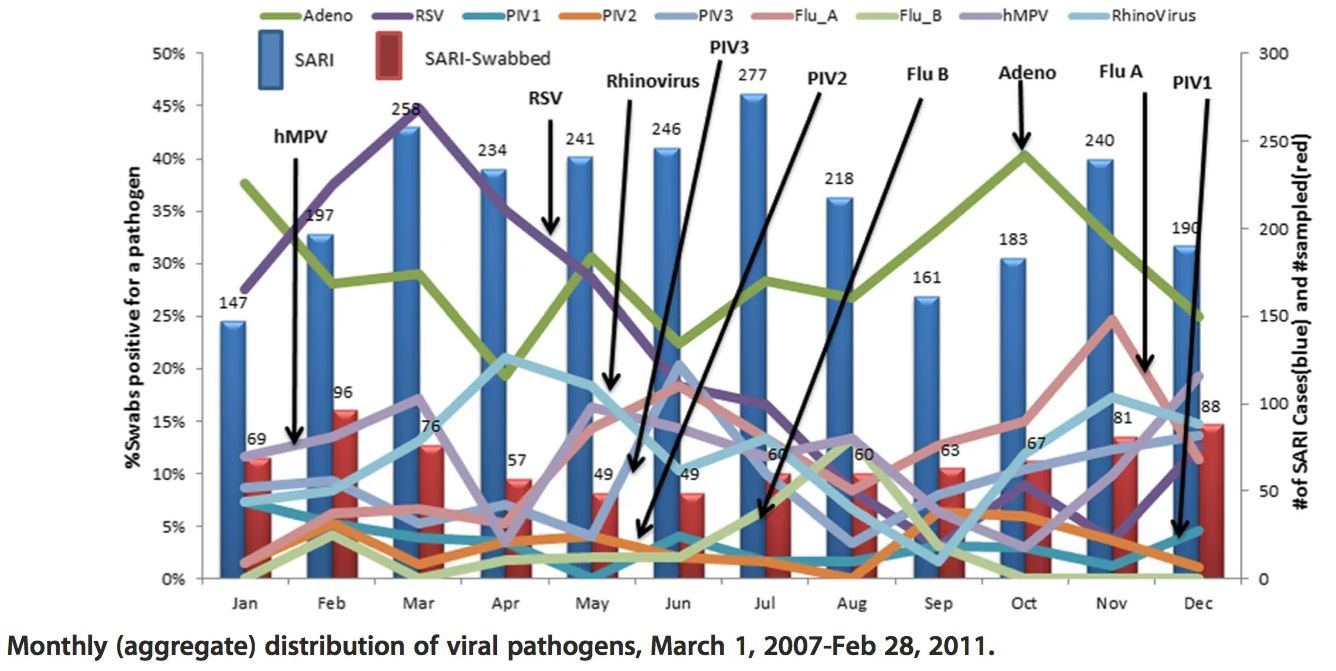
\includegraphics[width=1.0\textwidth]{ClutterredChart.jpg}
\end{center}
\end{frame}

\begin{frame} % Cover slide
\frametitle{\textcolor{brique}{[-  \textbf{Designing for Humans}   -]}}
\begin{center}
\begin{itemize}[<+->]
  \only<1-3>{  Choice of Graphical encoding is important}
 % \only<2>{ 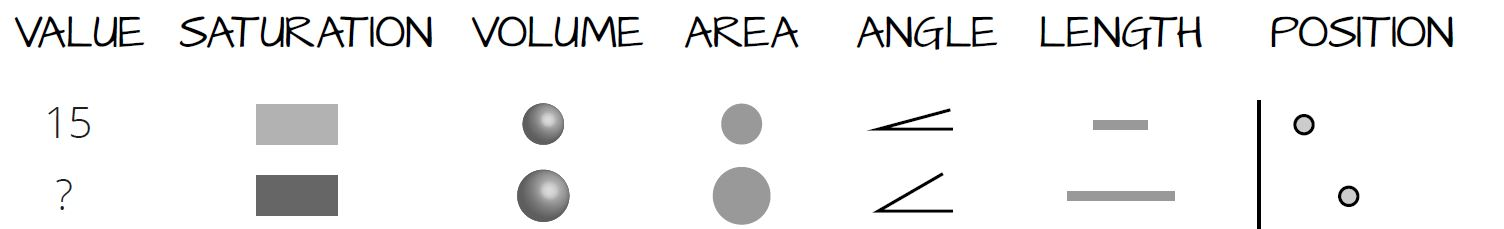
\includegraphics[width = 1.0\textwidth]{7visualEncoding.jpg}}
  \only<1-3>{  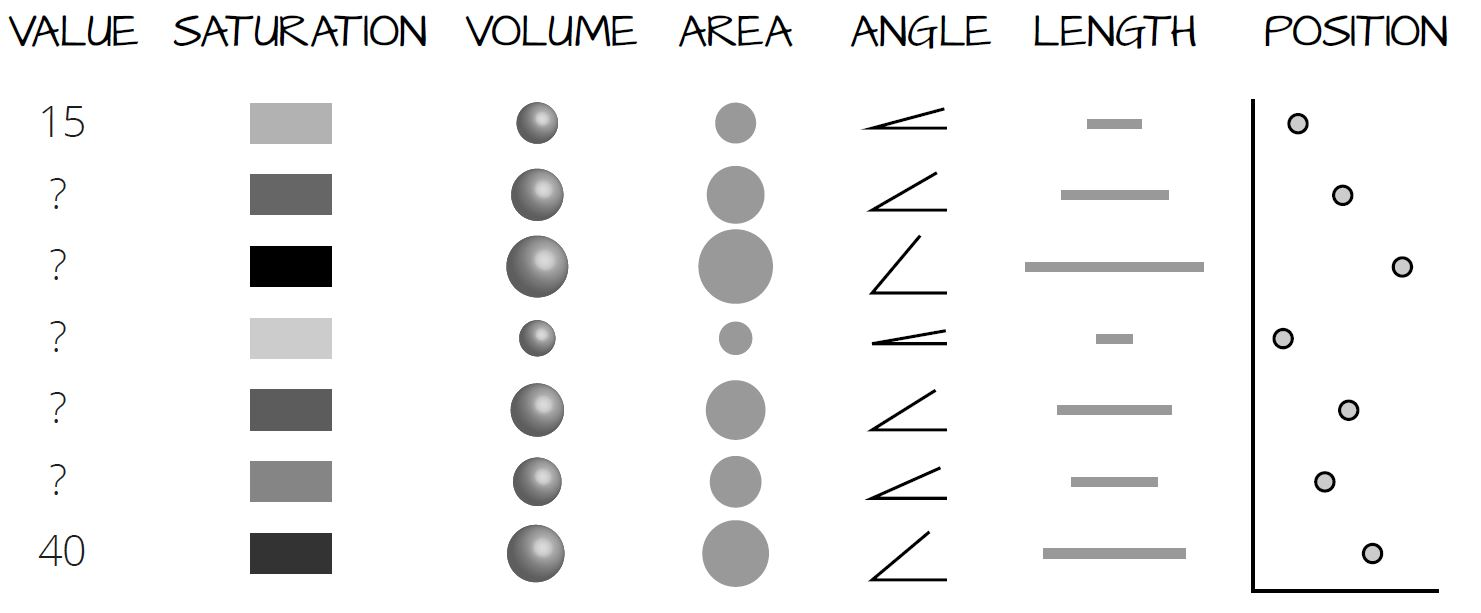
\includegraphics[width = 0.9\textwidth]{7visualEncodingFull.jpg} }
  \only<2-3>{ Answers are:}
  \only<3>{\textbf{15}, 30, 50, 10, 32, 24, \textbf{40}}
   \end{itemize}
\end{center}
\end{frame}
% Answers are 15, 30, 50, 10, 32, 24, 40.

\begin{frame} % Cover slide
\frametitle{\textcolor{brique}{[-  \textbf{Consider human limitations}   -]}}
\begin{center}
Modern graphics evolve fast but not  human visual system \\
\begin{tabular}{ll}
  \multirow{13}{*}{\includegraphics[width = 0.3\textwidth]{cleveland-McGill.png}}
                     & \\
                     & \textbf{Rank is:}\\
                     & \\
                     & 1-Position (aligned) \\
                     & 2- Position (non- aligned)\\
                     & 3- Length \\
                     & 4- Direction, angle \\
                     & 5- Area \\
                     & 6- Volume \\
                     & 7- Shading and saturation \\
                     & 8 - Color\\
                     & \\
                     & \hfill \textcolor{gris}{\footnotesize{From \cite{Cleveland1984}}} \\
  \end{tabular}
\end{center}
\end{frame}

\begin{frame} % Cover slide
\frametitle{\textcolor{brique}{[-  \textbf{Consider human limitations: A test}   -]}}
\begin{center}
    \begin{itemize}[<+->]
      \only<1-2>{ What percentage of the total area does the \textbf{black} surface represent? \\ }
      \only<2>{  \href{https://observablehq.com/d/af457a6ad31657f2}{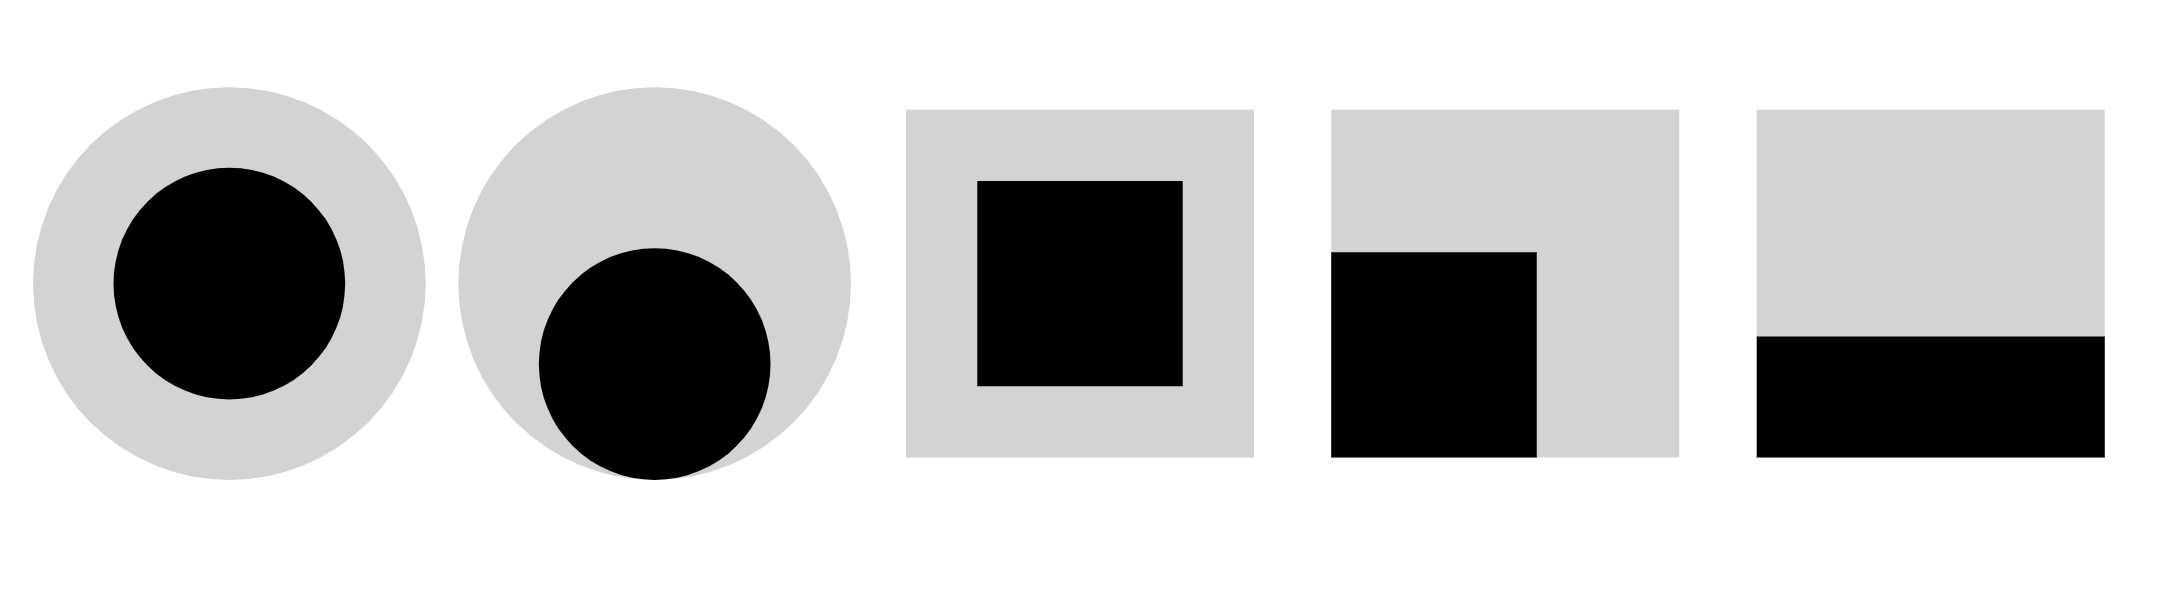
\includegraphics[width = 1.0\textwidth]{SurfaceWidget35.png} }}
      \only<3>{ And here? \\}
      \only<3>{  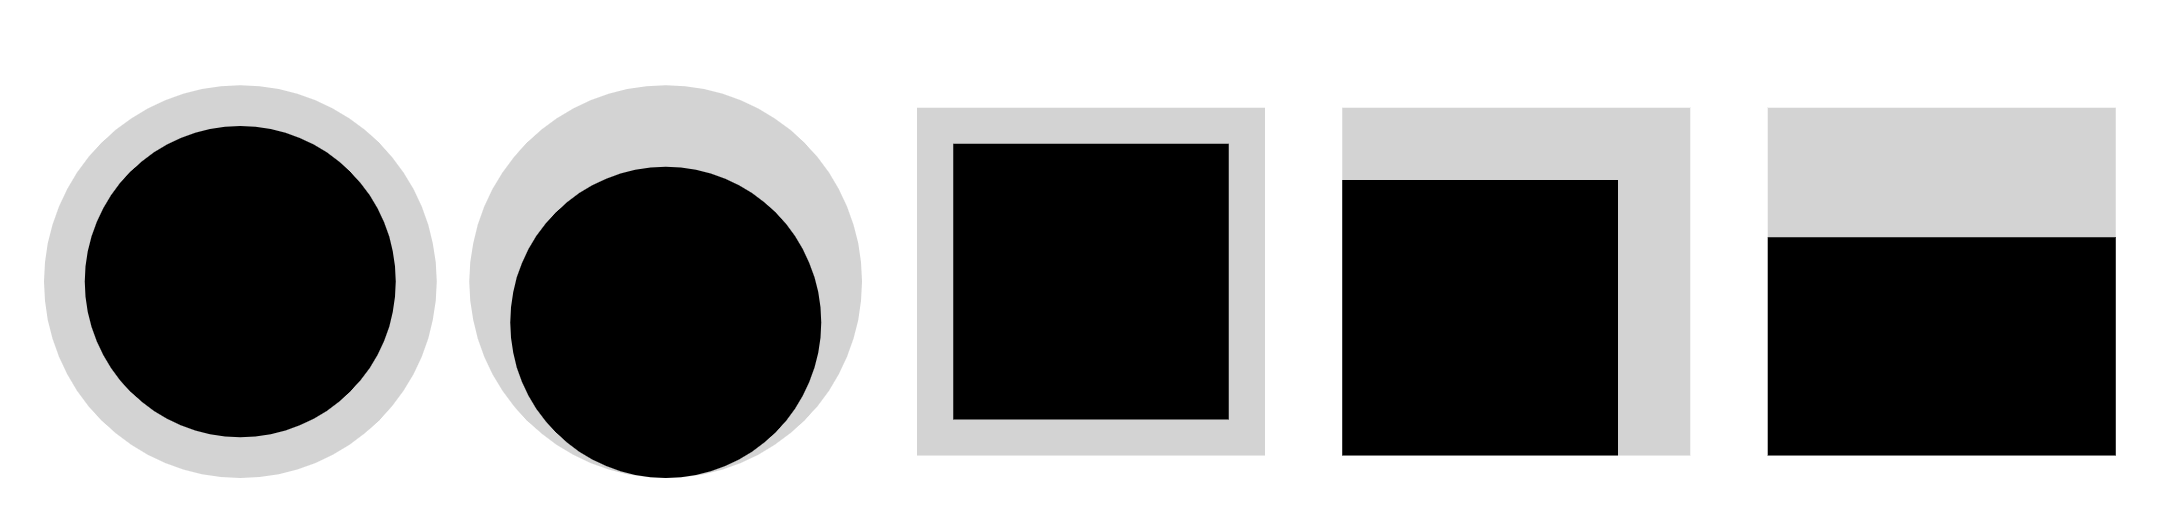
\includegraphics[width = 1.0\textwidth]{SurfaceWidget63.png} }
      \only<2-3>{ More examples on the \textcolor{siap}{\href{https://observablehq.com/d/af457a6ad31657f2}{interactive simulation widget}} }
       \only<4>{ 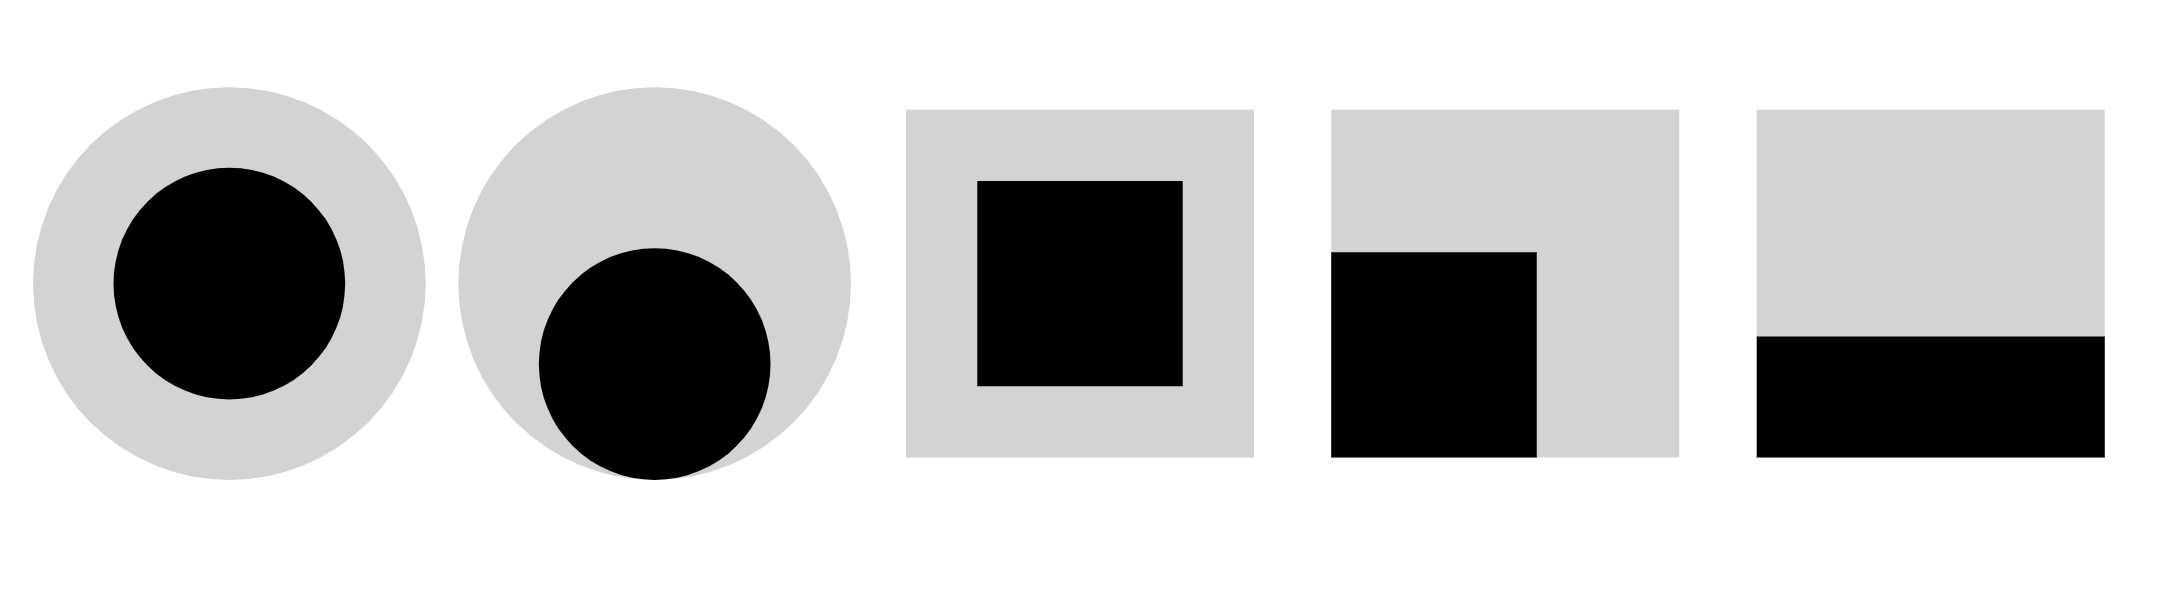
\includegraphics[width = 1.0\textwidth]{SurfaceWidget35.png} \\
         \hfill {\Large $\hookrightarrow$  35 \% } } 
     \only<5>{ 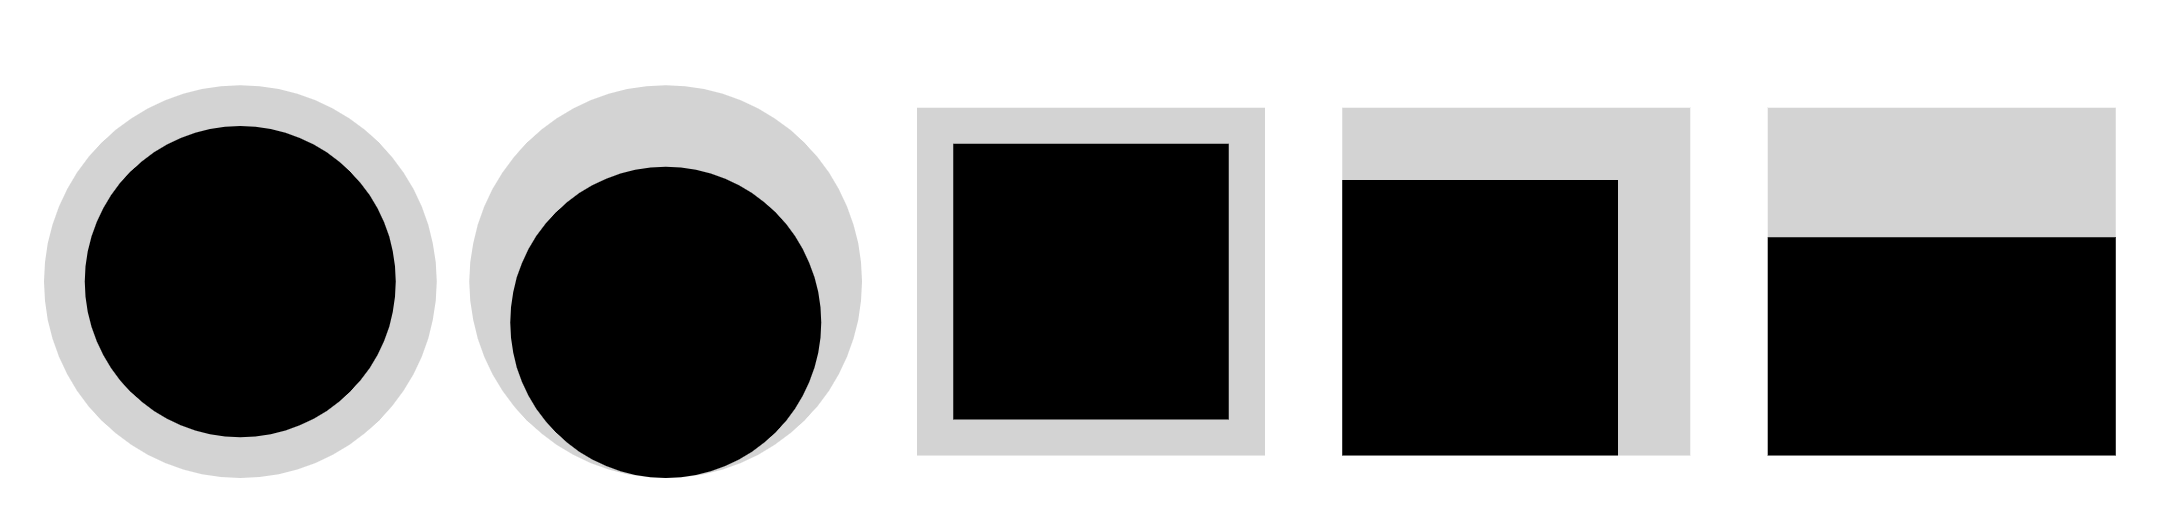
\includegraphics[width = 1.0\textwidth]{SurfaceWidget63.png}  \\
         \hfill {\Large $\hookrightarrow$  63 \% } } 
   \end{itemize}
\end{center}
\end{frame}

\section{Some Rules}


\begin{frame} % Cover slide
\frametitle{\textcolor{brique}{[- Good graphics? -]}}
%It the excellent Handbook of data visualisation \cite{Chen2007}, we find some good questions:
 \begin{itemize}
    \item<+->  What to Whom, How and Why ? \\
    %\emph{A graphic may be linked to three pieces of text: its \textbf{caption}, a \textbf{headline} and \textbf{an article} it accompanies. Ideally, all three should be consistent and complement each other.}
    \item<+->  Present or explore data?\\
  % \emph{ Different purpose, different requirements !}
    \item<+-> Choice of Graphical form ?\\
     %\emph{ Choice depends on the type of data to be displayed (e.g. univariate continuous data, bivariate categorical data, etc..) and on what is to be shown.}
    \item<+-> Unique solution? \\
   %\emph{ There is \textbf{not }always a unique optimal choice and alternatives can be equally good or good in different ways, emphasizing different aspects of the same data.}
 \end{itemize}
\end{frame}

%

%\section{Tufte's rules}

\begin{frame} % Cover slide
\frametitle{\textcolor{brique}{\textit{Edward R. Tufte'}s Rules}}
%In his seminal book, \cite{Tufte2001} propose some principles  for displaying quantitative information.
    \begin{enumerate}
       \item<+->[] \textbf{Data:} \emph{Above all, \textbf{show the data}}
       \item<+->[]\textbf{Question:} \emph{ Encourage the eye to compare different piece of data.}
       \item<+->[]\textbf{Data-ink ratio:} \emph{Maximize the \textbf{data-ink ratio}.}
       \item<+->[]\textbf{Integrity:} \emph{\textbf{Avoid distorting} what the data have to say}
      \item<+->[]\textbf{General to specific:} \emph{Reveal the data at \textbf{different levels of detail}}
      \item<+->[]\textbf{Context:}  \emph{Provide \textbf{statistical and verbal descriptions} of the data set.}
    \end{enumerate}
\end{frame}


\subsection{Data-ink ratio}

\begin{frame} % Cover slide
\frametitle{Data-Ink ratio}
\begin{center}
\emph{``Perfection is achieved not when there is nothing more to add, \\
but when there is nothing left to take away'' }
\end{center}
\flushright \emph{ Antoine de Saint-Exupery}
\end{frame}



\begin{frame} % Cover slide
\frametitle{\textcolor{brique}{[- Maximize Data-Ink Ratio -]}}
\begin{center}
\begin{itemize}
    \only<1>{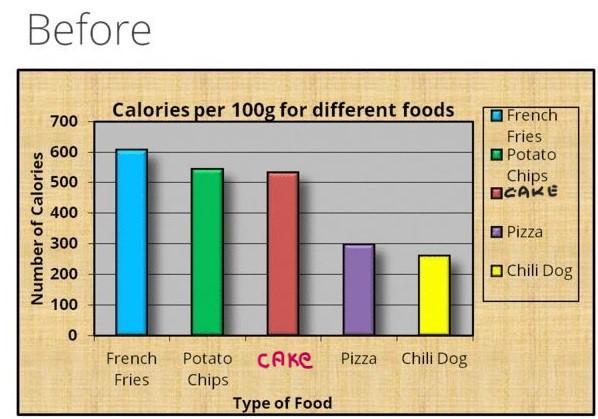
\includegraphics[width = 0.8\textwidth]{M2-Data-Ink-Ratio-Barsbefore.JPG} \\ }
    \only<2>{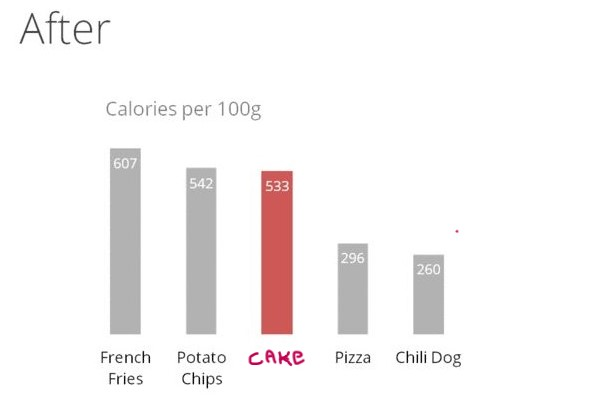
\includegraphics[width = 0.8\textwidth]{M2-Data-Ink-Ratio-BarsAfter.JPG} \\ }
    \only<1-2>{ \textcolor{gris}{\footnotesize{Source: \href{https://www.darkhorseanalytics.com/blog/data-looks-better-naked}{DarkHorse Analytics}}}}
\end{itemize}
\end{center}
\end{frame}


\begin{frame} % Cover slide
\frametitle{\textcolor{siap}{Have we lost something ?} }
\begin{figure}[h]
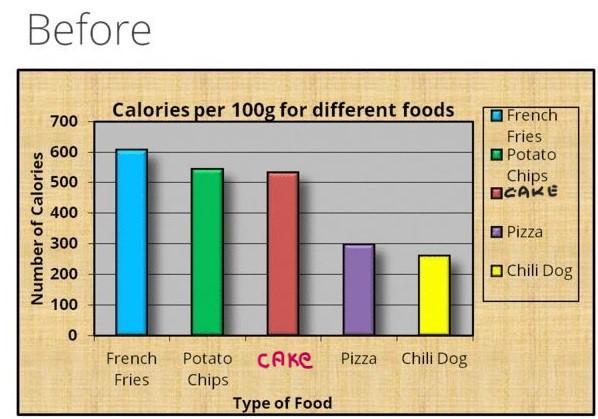
\includegraphics[width = 0.45\textwidth]{M2-Data-Ink-Ratio-Barsbefore.JPG}
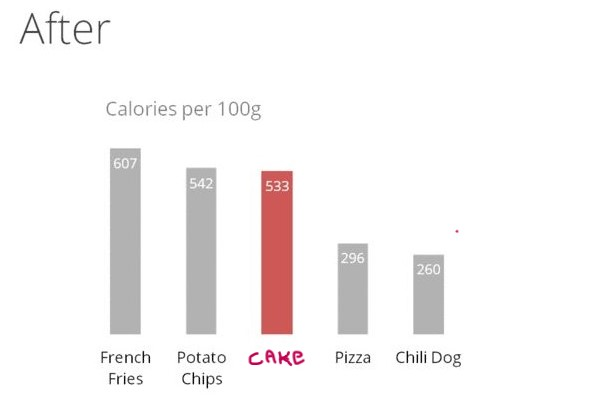
\includegraphics[width = 0.45\textwidth]{M2-Data-Ink-Ratio-BarsAfter.JPG}
\end{figure}
%Did you noticed that group 1 and group 3 had the same median (4.0)?
% see the \textit{ggplot} theme \texttt{+ theme\_tufte() }
%http://rpackages.ianhowson.com/cran/ggthemes/
\end{frame}


\subsection{Lie factor}
\begin{frame} % Cover slide
\frametitle{\textcolor{brique}{[- Integrity : The lie factor-]}}
\begin{equation}
Lie Factor = \frac{Size\;  of\; effect\;shown \; in \; graphic}{Size \; of\; effect \; in \; data}
\end{equation}
A Lie Factor $\neq$ 1 indicates a substantial distortion\\
$\hookrightarrow $ Deceptive or misleading visualization!!
\end{frame}

\begin{frame} % Cover slide
\frametitle{\textcolor{brique}{[- Integrity : The lie factor-]}}
\begin{figure}[h]
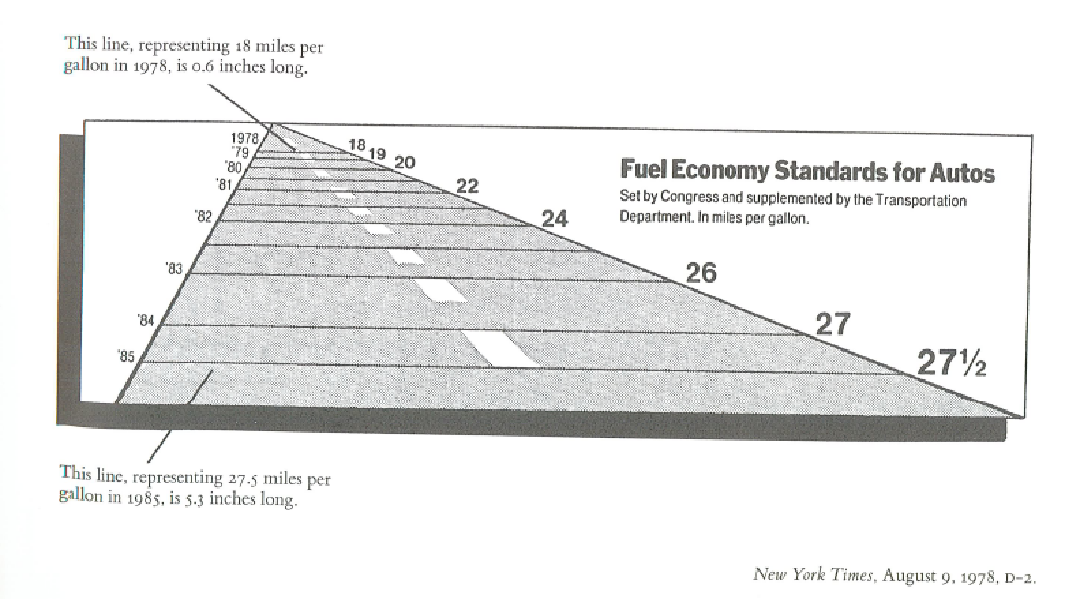
\includegraphics[width = 0.85\textwidth]{FuelEconomy1.pdf}
\caption{Fuel economy standards.}
\end{figure}
 \textcolor{gris}{\footnotesize{Source:  \cite{Tufte2001}  - from NY Times (1978)}}
\end{frame}

\begin{frame}
\frametitle{\textcolor{brique}{[- Integrity : The lie factor-]}}
\begin{figure}[h]
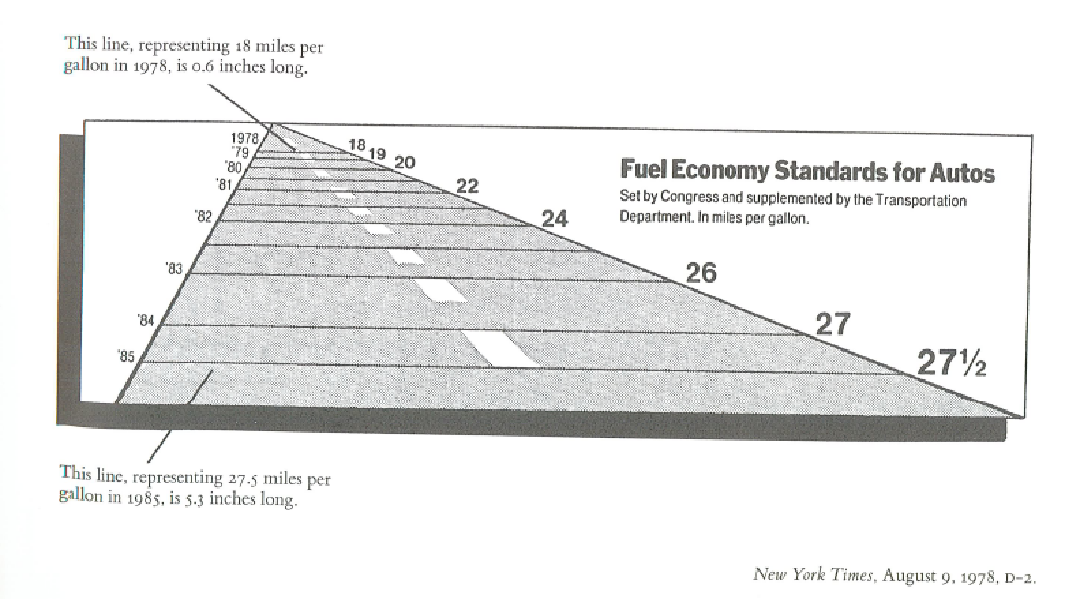
\includegraphics[width = 0.5\textwidth]{FuelEconomy1.pdf}
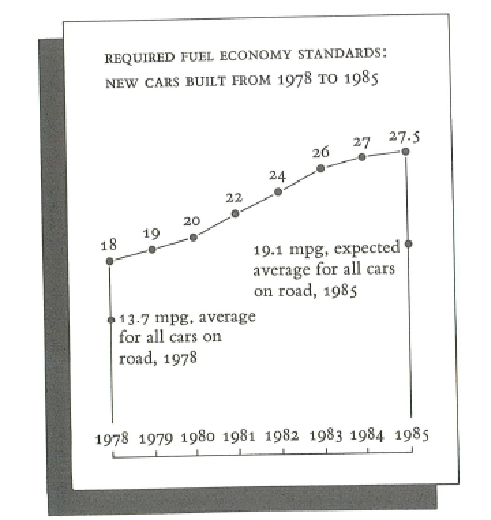
\includegraphics[width = 0.4\textwidth, angle =-1]{FuelEconomy2.pdf}
\caption{Fuel economy standards (revisited)}
\end{figure}
The "18 mpg" line measures  1.5 cm (in 1978) while "27,5 mpg" is represented by a 13 cm line (in 1985) \\
$\longrightarrow$ Lie factor =14.8 !
\end{frame}

\subsection{General to Specific}
\begin{frame}
\frametitle{\textcolor{brique}{[- From general to Specific -]}}
\begin{center}
\begin{itemize}
    \only<1>{ \centering 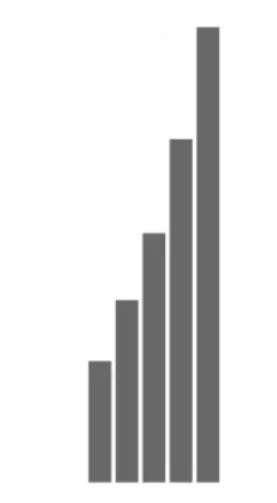
\includegraphics[width = 0.2\textwidth]{LimitedScopePartial-FR.jpg} \\ }
    \only<1>{ \centering Focusing can be misleading }
    \only<2>{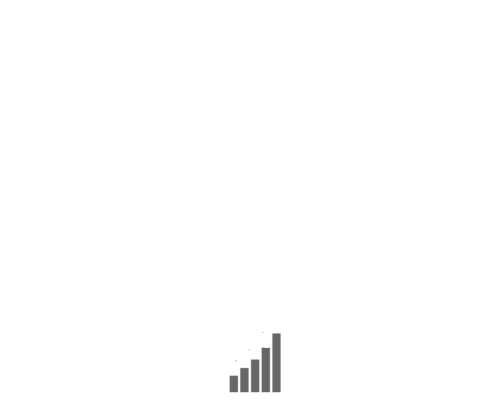
\includegraphics[width = 0.7\textwidth]{Limited-scope-FR.Empty.png} \\ }
    \only<3>{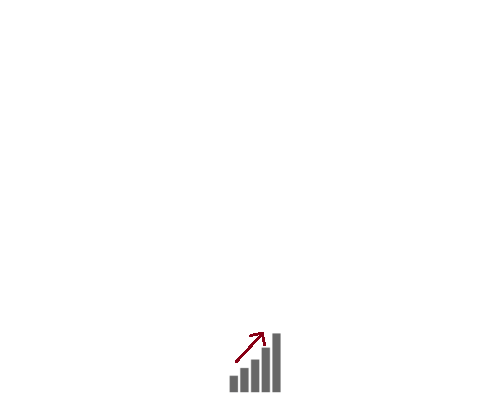
\includegraphics[width = 0.7\textwidth]{Limited-scope-FR.EmptyArrow.png} \\ }
    \only<2-3>{The big picture \textbf{may} be more interesting}
    \only<4>{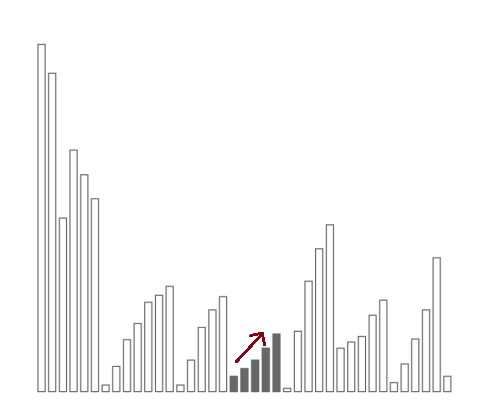
\includegraphics[width = 0.7\textwidth]{Limited-scope-FR-BigPicture.png} \\ }
    \only<4>{The big picture \textbf{is} more interesting}
\end{itemize}
\end{center}
\end{frame}

%%%%%%%%%%%%%  Context %%%%%%%ù
\begin{frame}
\frametitle{\textcolor{brique}{Exercise:} Compare 2 numbers }

In the next \textcolor{brique}{\textbf{5 minutes}}, you will design \textbf{``the best way''} to {\color{brique}\textbf{compare}} two numbers\\

\begin{itemize}[<+-|alert@+>]
    \item[]
    \item[] \begin{center}
            {\huge \textbf{75}} and {\huge \textbf{37}}.\\
            \end{center}
    \item[]  Use your imagination
\end{itemize}
\end{frame}


\begin{frame}
\frametitle{\textcolor{brique}{Exercise:} Context matters! }
\begin{itemize}
 \item[]
\only<1>{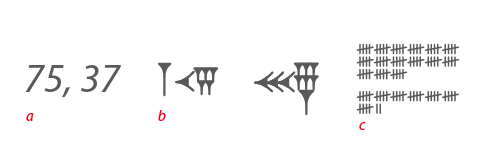
\includegraphics[height=3cm]{DesignNumbers-01.png}}
\only<2>{
\includegraphics[height=3cm]{DesignNumbers-02.png}}
\only<3>{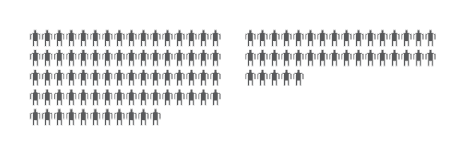
\includegraphics[height=3cm]{DesignNumbers-03.png}}
\only<4>{
\includegraphics[height=3cm]{DesignNumbers-04.png}}
\only<5>{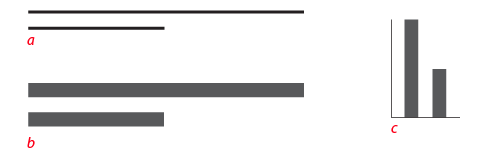
\includegraphics[height=3cm]{DesignNumbers-05.png}}
\only<6>{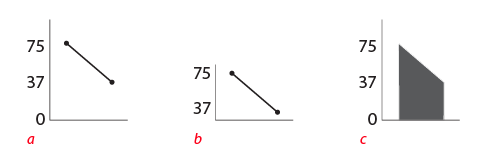
\includegraphics[height=3cm]{DesignNumbers-06.png}}
\only<7>{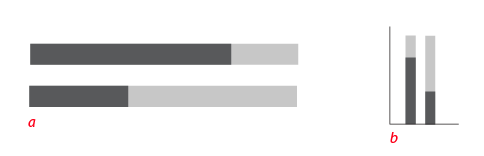
\includegraphics[height=3cm]{DesignNumbers-07.png}}
\only<8>{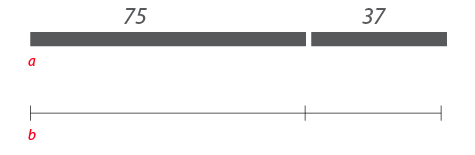
\includegraphics[height=3cm]{DesignNumbers-08.png}}
\only<9>{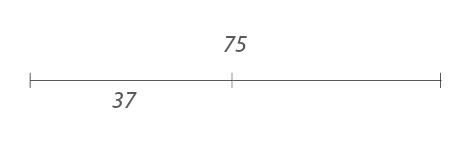
\includegraphics[height=3cm]{DesignNumbers-09.png}}
\only<10>{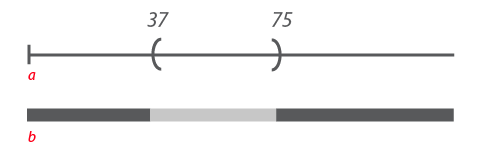
\includegraphics[height=3cm]{DesignNumbers-10.png}}
\only<11>{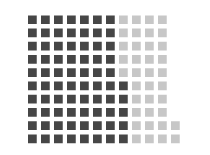
\includegraphics[height=4cm]{DesignNumbers-11.png}}
\only<12>{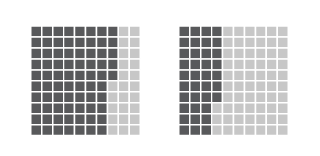
\includegraphics[height=4cm]{DesignNumbers-12.png}}
\only<13>{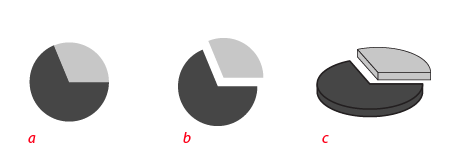
\includegraphics[height=3cm]{DesignNumbers-13.png}}
\only<14>{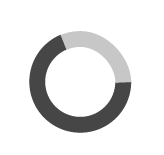
\includegraphics[height=4cm]{DesignNumbers-14.png}}
\only<15>{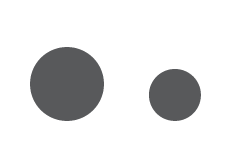
\includegraphics[height=4cm]{DesignNumbers-15.png}}
\only<16>{
\includegraphics[height=4cm]{DesignNumbers-16.png}}
\only<17>{
\includegraphics[height=4cm]{DesignNumbers-17.png}}
\only<18>{\includegraphics[height=4cm]{DesignNumbers-18.png}}
\only<19>{\includegraphics[height=4cm]{DesignNumbers-19.png}}
\only<20>{\includegraphics[height=4cm]{DesignNumbers-20.png}}
\only<21>{\includegraphics[height=4cm]{DesignNumbers-21.png}}
\only<22>{\includegraphics[height=4cm]{DesignNumbers-22.png}}
\only<23>{\includegraphics[height=4cm]{DesignNumbers-23.png}}
\only<24>{\includegraphics[height=3cm]{DesignNumbers-24.png}}
\only<25>{\includegraphics[height=3cm]{DesignNumbers-25.png}}
\only<26>{\includegraphics[height=4cm]{DesignNumbers-26.png}}
\only<27>{\includegraphics[height=4cm]{DesignNumbers-27.png}}
\only<28>{\includegraphics[height=4cm]{DesignNumbers-28.png}}
\only<29>{\includegraphics[height=4cm]{DesignNumbers-29.png}}
\only<30>{\includegraphics[height=4cm]{DesignNumbers-N1.jpg}}
%\only<31>{\includegraphics[height=4cm]{DesignNumbers-N2.jpg}}
\end{itemize}

\vfill
\textit{Adapted from} \href{https://visual.ly/blog/45-ways-to-communicate-two-quantities/}{\textit{S. Ortiz}}
\end{frame}



--------------------
% the \setbeamercolor and the frame to limit the scope
{\setbeamercolor{background canvas}{bg=siap}
 \setbeamercolor{item}{fg=white}
    \setbeamercolor{normal text}{fg=white}
    \usebeamercolor[fg]{normal text}
\begin{frame}
\hspace{4cm}
\begin{center}
\Huge{Graphics for Big Data}
\end{center}
\end{frame}

} %end blue Background -------------------

\section{Parallel Coordinates }

%%% Parallel coordinates

\begin{frame} % Cover slide
\frametitle{\textcolor{brique}{[-  \textbf{Parallel Coordinates Plots}   -]}}
\begin{center}
\begin{enumerate}
   \only<1>{\includegraphics[width = 0.8\textwidth]{ParallelCoord_BBach1.png} \\ }
   \only<2>{\includegraphics[width = 0.8\textwidth]{ParallelCoord_BBach2.png}\\ }
   \only<3>{\includegraphics[width = 0.8\textwidth]{ParallelCoord_BBach3.png} \\ }
   \only<4>{\includegraphics[width = 0.8\textwidth]{ParallelCoord_BBach4.png}\\ }
   \only<1-4>{\textcolor{gris}{\tiny{From \cite{wang2020}. PCP invented in  1959 by \href{https://en.wikipedia.org/wiki/Alfred_Inselberg}{Alfred Inselberg}.}}}
\end{enumerate}
\end{center}
\end{frame}


\begin{frame} % Cover slide
\frametitle{\textcolor{brique}{[-  \textbf{Parallel Coordinates properties}   -]}}
\begin{figure}[h]
\includegraphics[width = 0.8\textwidth]{ParallelCoordinatesGroups.pdf}
\end{figure}
\textcolor{gris}{From  \cite{Unwin2006}}
\end{frame}



\begin{frame} % Cover slide
\frametitle{\textcolor{brique}{[-  \textbf{Parallel Coordinates: Application}   -]}}
\begin{center}
\begin{enumerate}
   \only<1>{\includegraphics[width = 1.0\textwidth]{ParallelGblack-1.png}}
   \only<2>{\includegraphics[width = 1.0\textwidth]{ParallelGrey-1.png}}
   \only<3>{\includegraphics[width = 1.0\textwidth]{ParallelG1-1.png}}
   \only<4>{\includegraphics[width = 1.0\textwidth]{ParallelSpecific-1.png}}
   % captures dynamic version
   %\only<5>{\includegraphics[width = 1.0\textwidth]{ParallelCoord_BBach4.png}}
\end{enumerate}
\end{center}
\end{frame}

\section{Interactivity}


\begin{frame} % Cover slide
\frametitle{\textcolor{brique}{[-  \textbf{Parallel Coordinates + Interactivity}   -]}}
\begin{center}
\begin{enumerate}
   \only<1>{\includegraphics[width = 1.0\textwidth]{M4-ParallelSDGCountries0.png}}
   \only<2>{\includegraphics[width = 1.0\textwidth]{M4-ParallelSDGCountries1.png}}
   \only<3>{\includegraphics[width = 1.0\textwidth]{M4-ParallelSDGCountries2.png}}
   \only<4>{\includegraphics[width = 1.0\textwidth]{M4-ParallelSDGCountries3.png}}
   \only<5>{\includegraphics[width = 1.0\textwidth]{M4-ParallelSDGCountries4.png}}
   \only<6>{\includegraphics[width = 1.0\textwidth]{M4-ParallelSDGCountries5.png}}
   % captures dynamic version
   %\only<5>{\includegraphics[width = 1.0\textwidth]{ParallelCoord_BBach4.png}}
\end{enumerate}
\end{center}
\end{frame}



\begin{frame} % Cover slide
\frametitle{\textcolor{brique}{[-  \textbf{Slope graph}  -]}}
\begin{center}
\begin{itemize}
   \only<1-3>{Comparing the evolution of an indicator between two periods  \\ }
   \only<2-3>{Sometimes easier to simplify the view when many observations \\ }
   \only<3>{Taking the first and last points, simplifies the message \\ } %Big picture first
   \only<4>{\includegraphics[width = 0.6\textwidth]{slope1-1.png} \\ }
   \only<5>{ \includegraphics[width = 0.6\textwidth]{slope2-1.png} \\ }
   \only<6>{Using some \textcolor{brique}{pre-attentive} variables to highlight increases \\
   \medskip
   \includegraphics[width = 0.45\textwidth]{slope1-1.png}
\includegraphics[width = 0.45\textwidth]{slope2-1.png} }
\end{itemize}
\end{center}
\end{frame}


\section{Storytelling}

% the \setbeamercolor and the frame to limit the scope
{\setbeamercolor{background canvas}{bg=siap}
 \setbeamercolor{item}{fg=white}
    \setbeamercolor{normal text}{fg=white}
    \usebeamercolor[fg]{normal text}

\begin{frame}
\hspace{4cm}
\begin{center}
\Huge{Storytelling with Data}
\end{center}
\end{frame}

} %end blue Background


\begin{frame} % Cover slide
\frametitle{\textcolor{brique}{[-  \textbf{Telling a story} -]}}
\begin{center}

\begin{itemize}
  \only<1>{ \center \Large \textcolor{brique}{\textbf{Visual}} communication \\ is different from \\ \textcolor{brique}{\textbf{Text}} communication \\ }
  \only<2-3>{ $\hookrightarrow$   For the reader, a text is linear, a graphic is not! \\ }
  \only<2-3>{ \begin{tabular}{ccc}
     && \includegraphics[width = 0.35\textwidth]{TextReadingTime.JPG}  \\
     \includegraphics[width = 0.20\textwidth]{TextReading.JPG} & & \includegraphics[width = 0.20\textwidth]{TextReading2.JPG}
            \end{tabular} }
  \only<4>{ This affects the message, attention and perception \\ }
  \only<5>{ $\hookrightarrow$  Designers know this... \\ }
  \only<5>{ \includegraphics[width = 0.5\textwidth]{ReadThisFirst.png} \\  }
  \only<5>{\textcolor{gris}{\footnotesize{From \href{https://twitter.com/SteveStuWill/status/1499776684093960196?s=20}{ Steve Stewart-Williams (twitter)}}}}
\end{itemize}
\end{center}
\end{frame}

\begin{frame} % Cover slide
\frametitle{\textcolor{brique}{[-  \textbf{Visual Stories } -]}}
\begin{center}

\begin{itemize}
  \only<1>{\center  \Large  With graphics, \\the \textbf{reader} constructs the story}
  \only<2>{ \center  \Large  Reading is \textcolor{brique}{\textbf{not linear}} \\  }
  \only<3>{\center It is a \textbf{reader-based} story  \\  }
  \only<3>{ \center \includegraphics[width = 0.35\textwidth]{SmallMultiplePaper.JPG} \\  }
  \only<4-5>{ \center The \textbf{story} changes with the  \textbf{graphic} }
   \only<5>{ The \emph{Area Of Interest} (AOI, in orange) \\  }
  \only<5>{\includegraphics[width = 0.7\textwidth]{BarvsWeb.JPG} \\}
  \only<6>{ \textbf{8} different ways of presenting the same information \\ }
  \only<6>{\includegraphics[width = 0.7\textwidth]{EightWaysSameData.JPG} \\ }
  \only<7-9>{ Eyes Trajectories  (eyes-tracking)\\ }
  \only<7-9>{\includegraphics[width = 0.45\textwidth]{EyeTracking.JPG} \\ }
  \only<7>{ $\rhd$ Not the same  \textbf{trajectories}\\  }
  \only<8>{ $\rhd$ Not the same \textbf{efficiency} (Time, accuracy,  comparisons) \\ }
  \only<9>{ $\rhd$ Not the same \textbf{story}\\ }
 % \only<10>{ $\rhd$ Time to get information differs\\ }
%  \only<10>{\includegraphics[width = 0.6\textwidth]{ResultsGoldberg2010.JPG} \\}
%  \only<10>{ \emph{Linear graphs} provide information faster\\  }
  \only<5-10>{ \textcolor{gris}{\footnotesize{From  \cite{goldberg2010}}} \\  }
\end{itemize}
\end{center}
\end{frame}


\begin{frame} % Cover slide
\frametitle{\textcolor{brique}{[-  \textbf{\emph{"Scrolly"}telling } -]}}
\begin{center}
\begin{itemize}[<+->]
   \only<1-3>{ \center \large \textcolor{siap}{"\textbf{Scrollytelling}"} is a composite answer \\  \vspace{1cm} }
   \only<2-3>{$\hookrightarrow$ Facilitates the narrative for complex data \\ }
   \only<3>{$\hookrightarrow$ Text drives the narration\\  }
   \only<4-6>{1- Guided reading $\hookrightarrow$ Teach how to read \\ }
   \only<5>{  \href{https://flourish.studio/blog/international-womens-day/}{\includegraphics[width = 0.7\textwidth]{WomenInParliament-Flourish.png}} \\ }
   \only<7>{2-  Free navigation $\hookrightarrow$  Explore (read)  yourself \\}
   \only<7>{ \href{https://flourish.studio/blog/international-womens-day/}{ \includegraphics[width = 0.7\textwidth]{SlopeGenderCarreers2.png}} \\ }
   \only<5-7>{\hfill \textcolor{gris}{\footnotesize{From
    \href{https://flourish.studio/blog/international-womens-day/}{Gender Inequality Statistics 2024 - Flourish}  }}}
    \only<8>{ \textcolor{siap}{\Large   $\hookrightarrow$ Build your \textbf{own} story! }}
\end{itemize}
\end{center}
\end{frame}

%SlopeGenderCarreers.png
%WomenFortune.png

\section{Ethical DataViz}

% the \setbeamercolor and the frame to limit the scope
{\setbeamercolor{background canvas}{bg=siap}
 \setbeamercolor{item}{fg=white}
    \setbeamercolor{normal text}{fg=white}
    \usebeamercolor[fg]{normal text}

\begin{frame}
\hspace{4cm}
\begin{center}
\Huge{Ethical Data Visualisation}
\end{center}
\end{frame}

} %end blue Background


\begin{frame} % Cover slide
\frametitle{\textcolor{brique}{[- Ethical Visualization -]}}
\begin{center}
\begin{itemize}
   \only<1-4>{ \textcolor{siap}{\textbf{Ethical} principle: \textbf{Do Not Harm} } \\  }
   \only<2-3>{\includegraphics[width =0.4\textwidth]{WomenSizeIcon.png} \\}
   \only<3>{ \emph{As an Indian woman, (...) praying the terrifying gang of international
giant ladies (...) don't find me. \\ }}
   \only<2-3>{\hfill \textcolor{gris}{\footnotesize{Source:   \href{https://twitter.com/reina_sabah/status/1291509085855260672?lang=en}{@reina\_sabah} and \cite{Schwabish2022}  }}}
\end{itemize}
\end{center}
\end{frame}

\begin{frame} % Cover slide
\frametitle{\textcolor{brique}{[-\textbf{Bar chart can be misleading}-]}}
\begin{figure}
\includegraphics[width = 0.9\textwidth]{Truncated_Bar_Graph.png}
\end{figure}
\textcolor{gris}{\footnotesize{Source: \href{https://en.wikipedia.org/wiki/Misleading_graph}{Wikipedia: Misleading graph}}}  \hfill \textcolor{brique}{\textbf{Poll}}
\end{frame}

\begin{frame} % Cover slide
\frametitle{\textcolor{brique}{[-\textbf{Bar charts always start at 0}-]}}
\begin{figure}[h]
\includegraphics[width = 0.9\textwidth]{Bar_graph.png}
\end{figure}
\textcolor{gris}{\footnotesize{Source: \href{https://en.wikipedia.org/wiki/Misleading_graph}{Wikipedia: Misleading graph}}}
\end{frame}


\begin{frame} % Cover slide
\frametitle{\textcolor{brique}{[- Ethical Visualization -]}}
\begin{center}
\begin{itemize}
   \only<2-4>{ \textcolor{siap}{ \textbf{Ethical} principle: Avoid Stereotypes } \\  }
   \only<2>{$\hookrightarrow $  \emph{"deficit thinking"} \\ }
   \only<3>{\includegraphics[width =0.5\textwidth]{WaiterBar.png} \\}
    \only<4>{\includegraphics[width =0.5\textwidth]{WaiterPoints.png} \\}
    \only<5>{\includegraphics[width =0.7\textwidth]{bar-vs-jitter-exp1.png} \\}
     \only<5>{The bar chart exaggerates \textbf{group homogeneity} while \textbf{there is variation \emph{within}} the groups.}
   \only<3-5>{\hfill \textcolor{gris}{\footnotesize{Source:   \href{https://rojasblakely.com/what-can-go-wrong-racial-equity-dataviz-deficit-thinking/}{Pieta Blakely} }}}
\end{itemize}
\end{center}
\end{frame}

%The bar chart exaggerates group homogeneity because it gives no indication of the outcome variation within the groups. It only shows the outcome differences between the groups. This creates the false impression that all Asian people earn higher wages than all White, Hispanic and Black people, when in reality there’s considerable overlap (as you can see in the Jitter plot). Research shows that when people underestimate the variation of outcomes within a category, they overestimate the impact of the category on the outcome. That is, they’re more likely to falsely conclude “being Black causes lower wages.”

\begin{frame}
\frametitle{\textcolor{brique}{[- \textbf{Think of uncertainty! } -]}}
\begin{center}
\begin{itemize}
   \only<1>{What would be your decision based on this graphic? \\ }
   \only<1-2>{\includegraphics[width =0.9\textwidth]{TimeTrendMean.png} \\}
   \only<3>{ Now, what do you think? \\ }
   \only<3>{\includegraphics[width =0.9\textwidth]{TimeTrendbounds.png} \\}
   \only<4>{Many observations in  A  are below those of group B!}
  \only<4>{\includegraphics[width =0.9\textwidth]{TimeTrendPoints.png} \\}

\end{itemize}
\end{center}
\end{frame}

\begin{frame}
\frametitle{\textcolor{brique}{[- \textbf{Conclusion} -]}}
\begin{center}
\begin{itemize}[<+-|alert@+>]
\item Big data may need complex graphics
\item Complex graphics may be difficult to read
\item Complex graphics should allow for fair comparisons
\item Complex graphics should answer legitimate questions
\item Sometimes several simple graphics are better than one
\end{itemize}
\end{center}
\end{frame}


\begin{frame}
\frametitle{\textcolor{brique}{[- \textbf{Conclusion} -]}}
\begin{center}
\emph{“The greatest value of a picture is when it forces us \\ to notice what we never expected to see.”}\\

\hfill \cite{Tukey1977}
\end{center}
\end{frame}

\begin{frame} % Cover slide
\frametitle{\textcolor{brique}{[Q\&A]}}
\begin{center}
\Large \textcolor{siap}{ Questions}
\end{center}
\end{frame}


\begin{frame}[allowframebreaks]%in case more than 1 slide needed
\frametitle{References}
\nocite{Cairo2019}
\nocite{Correll2019}
\nocite{Allen2016}
\nocite{Isenberg2011}
\nocite{Kelleher2011}
\nocite{Tufte2001}
\nocite{Cleveland1982}
%\nocite{*}
    {\footnotesize
    %\bibliographystyle{authordate1}
    \bibliographystyle{apalike}
    \bibliography{Visu, VisuSeminal}
    }
\end{frame}

\end{document}

\begin{frame} % Cover slide
\frametitle{ }
\pause
 \begin{itemize}[<+->]
  \item[]
  \item
\end{itemize}
\end{frame}

%%%%%%%%%%%%%%% Last Slide %%%%%%%%%%%%%%%%



%\bibliographystyle{authordate1}
%\bibliography{c:/Chris/Visualisation/Visu}
%\end{frame}

\begin{frame}{Title}
\begin{columns}[T]
  \begin{column}{0.7\textwidth}
    \begin{itemize}[<+->]
        \item Sometimes data providers propose a more efficient way to download data
        \item API: "\textbf{A}pplication \textbf{P}rogramming \textbf{I}nterface "
        \item An API is like a waiter in a restaurant
        \item[$\hookrightarrow$ ] He has a menu
        \item[$\hookrightarrow$ ] You can order anything but only on the Menu
        \item[$\hookrightarrow$ ] Data is then served as a structured "ready-to-use" file
     \end{itemize}
     \end{column}

    \begin{column}{0.3\textwidth}
    \begin{center}
      \includegraphics[width=0.9\textwidth]{undraw_diet_ghvw.png}
    \end{center}
    \end{column}
\end{columns}
\end{frame}

